\documentclass[12pt,          % font size: 11pt or 12pt
               phd,           % degree:    ms or phd
               doublespacing % spacing: onehalfspacing or doublespacing
               ]{ncsuthesis}

%%----------------------------------------------------------------------------%%
%%------------------------------ Import Packages -----------------------------%%
%%----------------------------------------------------------------------------%%

\usepackage{booktabs}  % professionally typeset tables
\usepackage{amsmath}
\usepackage{amssymb}
\usepackage{textcomp}  % better copyright sign, among other things
\usepackage{xcolor}
\usepackage{lipsum}    % filler text
\usepackage{mathtools}
\usepackage{geometry}
\usepackage{graphicx}
\usepackage{relsize}
\usepackage{environ}
\usepackage{newlfont}
\usepackage{caption}
\usepackage{subcaption}
\usepackage{titlesec}
\usepackage[export]{adjustbox}
\usepackage[position=b]{subcaption}
\usepackage{url}
\urlstyle{same}


%%----------------------------------------------------------------------------%%
%%---------------------------- Formatting Options ----------------------------%%
%%----------------------------------------------------------------------------%%
%%

%% -------------------------------------------------------------------------- %%
%% Disposition format -- any titles, headings, section titles
%%  These formatting commands affect all headings, titles, headings,
%%  so sizing commands should not be used here.
%%  Formatting options to consider are
%%     +  \sffamily - sans serif fonts.  Dispositions are often typeset in
%%                    sans serif, so this is a good option. 
%%     +  \rmfamily - serif fonts
%%     +  \bfseries - bold face
%\dispositionformat{\sffamily\bfseries}   % bold and sans serif
\dispositionformat{\bfseries}            % bold and serif

%% -------------------------------------------------------------------------- %%
%% Formatting for centered headings - Abstract, Dedication, etc. headings
%%  This is where one might put a sizing command.
%%  \MakeUppercase can be used to typeset all headings in uppercase.
\headingformat{\large\MakeUppercase}   % All letters uppercase
%\headingformat{\large}                % Not all uppercase
%\headingformat{\Large\scshape}        % Small Caps, used with serif fonts.

%% Typographers recommend using a normal inter-word space after
%% sentences. TeX's default is to add an wider space, but \frenchspacing
%% gives a normal spacing. Comment out the following line if you prefer
%% wider spaces between sentences.


%% -------------------------------------------------------------------------- %%
%%  Optional packages
%%    A number of compatible packages to improve the look and feel of
%%    your document are available in the file optional.tex 
%%    (For example, hyperlinks, fancy chapter headings, and fonts)
%% To use these options, uncomment the next line and see optional.tex
\include{optional}


%%----------------------------------------------------------------------------%%
%%---------------------------- Content Options -------------------------------%%
%%----------------------------------------------------------------------------%%
%% Size of committee: 3, 4, 5, or 6 -- this number includes the chair
\committeesize{5}

%% Members of committee
%%  Each of the following member commands takes an optional argument
%%   to specify their role on the committee.
%%  For co-chairs, use the commands:
%%      \cochairI{Doug Dodd}
%%      \cochairII{Chris Cox}
%%
\cochairI{Hassan Hassan}
\cochairII{Peter Gnoffo}
\memberI{Jack Edwards}
\memberII{Hong Luo}
\memberIII{John Griggs}


%% Student writing thesis, \student{First Middle}{Last}
\student{Kyle B.}{Thompson} % a middle initial

%% Degree program
\program{Aerospace Engineering}

%% Thesis Title
%%  Keep in mind, according to ETD guidelines:
%%    +  Capitalize first letter of important words.
%%    +  Use inverted pyramid shape if title spans more than one line.
%%
%%  Note: To break the title onto multiple lines, use \break instead of \\.
\thesistitle{Aerothermodynamic Design Sensitivities for a Reacting Gas Flow Solver \break
on an Unstructured Mesh Using a 
Discrete Adjoint Formulation}

%% Degree year.  Necessary if your degree year doesn't equal the current year.
%\degreeyear{1995}


%%----------------------------------------------------------------------------%%
%%---------------------------- Personal Macros -------------------------------%%
%%----------------------------------------------------------------------------%%

\DeclareCaptionType{mycapequ}[][List of equations]
\captionsetup[mycapequ]{labelformat=empty}

\newcommand{\uv}[1]{\ensuremath{\mathbf{\hat{#1}}}}
\newcommand{\bo}{\ensuremath{\boldsymbol{\Omega}}}
\newcommand{\fref}[1]{Figure~\ref{#1}}
\newcommand{\frefs}[2]{Figure~(\ref{#1}-\ref{#2})}
\newcommand{\tref}[1]{Table~\ref{#1}}
\newcommand{\trefs}[2]{Tables~(\ref{#1}-\ref{#2})}
\newcommand{\eref}[1]{Eq.~\ref{#1}}
\newcommand{\erefs}[2]{Eq.s~(\ref{#1}-\ref{#2})}
\newcommand{\cref}[1]{Chapter~\ref{#1}}
\newcommand{\crefs}[2]{Chapters~(\ref{#1}-\ref{#2})}
\newcommand{\sref}[1]{section~\ref{#1}}
\newcommand{\pd}[2]{\frac{\partial #1}{\partial #2}}
\newcommand{\pnd}[3]{\frac{\partial^{#3} #1}{\partial #2^{#3}}}
\newcommand{\pdr}[3]{\left. \frac{\partial #1}{\partial #2}\right|_{#3}}

% Nondimensionalization macro
%\newcommand{\nondim}[1]{{#1}^{'}/{#1}_{ref}}

% Cost function target eqn
\newcommand{\cost}[1]{\left( {#1} - {#1}^{*} \right)}

% residual and its derivatives
\newcommand{\res}[1]{\vR_{#1}}
\newcommand{\resp}[1]{\vR_{#1}^{'}}
\newcommand{\resrho}{\sum_{i=1}^{N_s}\left(\vR_{\rho_i}\right)}

\newcommand{\rdiff}[2]{\pd{\vR_{#1}}{#2}}
\newcommand{\rpdiff}[2]{\pd{\vR^{'}_{#1}}{#2}}

\newcommand{\rlprod}[2]{\pd{\vR_{#1}}{#2} \adjlam{#1}}
\newcommand{\rlpprod}[2]{\pd{\vR^{'}_{#1}}{#2} \adjlam{#1}}

\newcommand{\tdiff}[2]{\pd{\vR_{#2}}{#1}}
\newcommand{\tpdiff}[2]{\pd{\vR_{#2}^{'}}{#1}}
\newcommand{\rtdiff}[2]{\pd{\vR_{#1}}{#2}^{\mathsmaller T}}

\newcommand{\drvdv}{\pd{\mathbf{\tilde{R}_{\mv}}}{\mv}}

% Sum with limits on top and bottom of sigma
\newcommand{\lsum}[3]{\sum\limits_{#1}^{#2}{#3}}

% Species sum
\newcommand{\ssum}{\sum\limits_{s=1}^{N_{ns}}}

% velocity magnitude (squared)
\newcommand{\qs}{u^2 + v^2 + w^2}
\newcommand{\qsp}{(u^{'})^2 + (v^{'})^2 + (w^{'})^2}

% adjoint lambda with subscript
\newcommand{\adjlam}[1]{\Lambda_{#1}}

% Equation sets
\newcommand{\ru}[1]{\res{{\mU}_{#1}}}
\newcommand{\rv}[1]{\res{{\mv}_{#1}}}

% specific heats
\newcommand{\cvs}{C_{v,s}}
\newcommand{\cps}{C_{p,s}}

% stoichiometric coefficients
\newcommand{\sprod}{\nu_{s,r}^{''}}
\newcommand{\sreact}{\nu_{s,r}^{'}}

% Roe average weighting
\newcommand{\roe}{\tilde{w}}

% fuel-air ratio for plenum
\newcommand{\fa}{\phi_p}

% plenum mass flow rate
\newcommand{\massflow}{\dot{m}_p}

\newcommand{\br}[1]{B_{#1}^{r}}

\newcommand{\real}{\mathbf R}
\newcommand{\rnn}{\real^{N \times N}}
\newcommand{\rmn}{\real^{M \times N}}
\newcommand{\diag}{\mbox{diag}}
\newcommand{\norm}{\mathbf{n}}
\newcommand{\Norm}{\mathbf{N}}
\newcommand{\vf}{\mathbf f}
\newcommand{\vF}{\mathbf F}
\newcommand{\Fhat}{\mathbf{\hat{F}}}
\newcommand{\vx}{\mathbf x}
\newcommand{\vc}{\mathbf c}
\newcommand{\vd}{\mathbf d}
\newcommand{\vy}{\mathbf y}
\newcommand{\vz}{\mathbf z}
\newcommand{\ve}{\mathbf e}
\newcommand{\me}{\mathbf E}
\newcommand{\mg}{\mathbf G}
\newcommand{\vw}{\mathbf w}
\newcommand{\mw}{\mathbf W}
\newcommand{\mr}{\mathbf R}
\newcommand{\mh}{\mathbf H}
\newcommand{\mc}{\mathbf C}
\newcommand{\ms}{\mathbf S}
\newcommand{\mi}{\mathbf I}
\newcommand{\vb}{\mathbf b}
\newcommand{\vq}{\mathbf q}
\newcommand{\va}{\mathbf a}
\newcommand{\vv}{\mathbf v}
\newcommand{\vu}{\mathbf u}
\newcommand{\vU}{\mathbf U}
\newcommand{\vR}{\mathbf R}
\newcommand{\Up}{\mathbf{U}'}
\newcommand{\Uhat}{\mathbf{\hat{U}}}
\newcommand{\ma}{\mathbf A}
\newcommand{\mb}{\mathbf B}
\newcommand{\md}{\mathbf D}
\newcommand{\vr}{\mathbf r}
\newcommand{\mm}{\mathbf M}
\newcommand{\ml}{\mathbf L}
\newcommand{\mU}{\mathbf U}
\newcommand{\ul}{\mathbf{U^L}}
\newcommand{\ur}{\mathbf{U^R}}
\newcommand{\mv}{\mathbf V}
\newcommand{\Vhat}{\mathbf{\hat{V}}}
\newcommand{\mP}{\mathbf P}
\newcommand{\mq}{\mathbf Q}
\newcommand{\mx}{\mathbf X}
\newcommand{\pbar}{\overline p}

%%---------------------------------------------------------------------------%%
\begin{document}

%%---------------------------------------------------------------------------%%
\frontmatter

%% ------------------------------ Abstract ---------------------------------- %%
\begin{abstract}

  An algorithm is described to efficiently compute aerothermodynamic design
sensitivities using a decoupled variable set.  In a conventional approach to
computing design sensitivities for reacting flows, the species continuity
equations are fully coupled to the conservation laws for momentum and energy. In
this algorithm, the species continuity equations are solved separately from the
mixture continuity, momentum, and total energy equations. This decoupling
simplifies the implicit system, so that the flow solver can be made
significantly more efficient, with very little penalty on overall scheme
robustness.  Most importantly, the computational cost of the point implicit
relaxation is shown to scale linearly with the number of species for the
decoupled system, whereas the fully coupled approach scales quadratically. Also,
the decoupled method significantly reduces the cost in wall time and memory in
comparison to the fully coupled approach. 

This decoupled approach for computing design sensitivities with the adjoint
system is demonstrated for inviscid flow in chemical non-equilibrium around a
re-entry vehicle with a retro-firing annular nozzle. The sensitivities of the
surface temperature and mass flow rate through the nozzle plenum are computed
with respect plenum conditions and verified against complex-variable
finite-difference.  The decoupled scheme significantly improved the
computational time and memory required to complete the optimization, making this
an attractive method for high-fidelity design of hypersonic vehicles.

\end{abstract}


%% ---------------------------- Copyright page ------------------------------ %%
%% Comment the next line if you don't want the copyright page included.
\makecopyrightpage

%% -------------------------------- Title page ------------------------------ %%
\maketitlepage

%% -------------------------------- Dedication ------------------------------ %%
\begin{dedication}
 \centering To my parents and friends.
\end{dedication}

%% -------------------------------- Biography ------------------------------- %%
\begin{biography}
The author was born on December 11th, 1990, in Willow Springs, North Carolina.
He recieved a B.S. in Aerospace Engineering from North Carolina State University
in 2012, and subsequently recieved his M.S. in Aerospace Engineering from North
Carolina State University in 2014.  After recieving his M.S., he began work in
the Aerothermodynamics branch of NASA Langley Research Center, via the Pathways
program.  He completed this disseration on adjoint-based optimization while
working at NASA Langley Research Center.
\end{biography}

%% ----------------------------- Acknowledgements --------------------------- %%
\begin{acknowledgements}
First, I would like to thank Dr. Peter Gnoffo, who has been an unending source
of support during my time NASA Langley Research Center.  I would like thank my
parents for all of their encouragement over the years, and their commitment to
seeing I be given the best opportunity to make the most of myself.  I would like
to thank my advisor, Dr. Hassan, for instilling in me a diligence to improve
myself and for mentoring me through many challenges.  I would like to thank Dr.
Jeff White in the Computational Aerosciences Branch at NASA Langley Research
Center for his advice on reacting flow simulation. I would like to thank the
Entry Systems Modeling Project within NASA's Game Changing Development Program
for their funding and support of this research.  Finally, I would like to
recognize the FUN3D team at NASA Langley Research Center, for their support and
availability to discuss many challenging problems I have encountered during the
course of my time at NASA.
\end{acknowledgements}

\thesistableofcontents

\thesislistoftables

\thesislistoffigures

\begin{center}
  \textbf{NOMENCLATURE}
\end{center}

\textbf{Roman Symbols}
\bigskip
\begin{tabbing}
  XXXXXXXXX \= \kill% this line sets tab stop
  $A,\ A_d,\ A_m$ \> Jacobian Matrices \\
  $a$ \> Speed of sound, $m/s$ \\
  $\mathbf{b}$, $\res{}$ \> Residual vector \\
  $B^{r}_{i}$ \> Equilibrium constant curve fit coefficients \\
  $c_s$ \> Species $s$ mass fraction \\
  $C$ \> Decoupled scheme chemical source term Jacobian \\
  $C_{f,r}$ \> Preexponential factor of reaction $r$ \\
  $C_{p,s}$ \> Specific heat at constant pressure of species $s$ \\
  $C_{v,s}$ \> Specific heat at constant volume of species $s$ \\
  $D$ \> Decomposed diagonal Jacobian matrix \\
  $dv_1,\ dv_2,\ dv_3$ \> Eigenvector components \\
  $e_s$ \> Internal energy of species $s$, $J/kg^3$ \\
  $E$ \> Total energy per unit mass, $J/kg^3$ \\
  $E_{f,r}$ Activation energy of reaction $r$ \\
  $F_\rho'$\> Decoupled scheme mixture mass flux \\
  $F_{\rho_s}'$\> Decoupled scheme mass flux of species $s$ \\
  $\mathbf{F},\ \mathbf{F}',\ \mathbf{\hat{F}}$ \> Flux vectors \\
  $k_{f,r}$ \> Forward reaction rate coefficient of reaction $r$ \\
  $k_{b,r}$ \> Backward reaction rate coefficient of reaction $r$ \\
  $K_{c,r}$ \> Equilibrium constant of reaction $r$ \\
  $M_s$ \> Molecular weight of species $s$ \\
  $ns$ \> Number of species \\
  $n_x$, $n_y$, $n_z$ \> Face unit normal vector components \\
  $N$ \> Face normal vector, $m^2$ \\
  $N_{nodes}$ \> Number of nodes \\
  $N_{nz}$ \> Number of non-zero off-diagonal entries in Jacobian \\
  $N_{nb}$ \> Number of neighbors around local node \\
  $O$ \> Decomposed off-diagonal Jacobian matrix \\
  $p$ \> Pressure, $N/m^2$ \\
  $q$ \> primitive variables \\
  $R_\rho$ \> Decoupled scheme constraint \\
  $R_{f,r}$ \> Forward reaction rate of reaction $r$ \\
  $R_{b,r}$ \> Backward reaction rate of reaction $r$ \\
  $R_u$ \> Universal Gas Constant, $J/kg^3$ \\
  $\mathbf{S}$ \> Face normal vector, $m^2$\\
  $\mathbf{U},\ \mathbf{U}',\ \mathbf{\hat{U}}$ \> Conservative variable vectors \\
  $\overline{U}$ \> Normal velocity, $m/s^2$ \\
  $u,\ v,\ w$ \> Components of velocity, $m/s$ \\
  $V$ \> Cell volume, $m^3$ \\
  $\roe$ \> Roe scheme weighting factor \\
  $w_i$ \> Composite cost function component weight \\
  $\mathbf{\hat{V}}$ \>  Decoupled variables vector \\
  $\mathbf{W}$ \> Chemical source term vector \\
  $\mathbf{x}$, $\mathbf{y}$, $\mathbf{z}$ \> Spatial coordinates \\
 \end{tabbing}

\textbf{Greek Symbols}
\begin{tabbing}
  XXXXXXXXX \= \kill% this line sets tab stop
  $\lambda_1,\ \lambda_2,\ \lambda_3$ \> Acoustic and convective eigenvalues \\
  $\lambda^-,\ \lambda^+$ \> Species flux effective eigenvalues \\
  $\Lambda$ \> Diagonal eigenvalue matrix \\
  $\phi$ \> flux limiter result \\
  $\phi_p$ \> plenum fuel-air ratio \\
  $\rho$ \> Mixture density, $kg/m^3$ \\
  $\rho_s$ \> Species $s$ density, $kg/m^3$ \\
  $\sprod$ \> Stoichiometric coefficient of product species $s$ in reaction $r$ \\
  $\sreact$ \> Stoichiometric coefficient of reactant species $s$ in reaction $r$ \\
  $\omega$ \> Chemical source term scaling factor \\
  $\omega_s$ \> Chemical source term of species $s$ \\
\end{tabbing}

\textbf{Subscripts}
\begin{tabbing}
  XXXXXXXXX \= \kill% this line sets tab stop
  $o$ \> Reference value \\
  $\infty$ \> Freestream condition \\
\end{tabbing}

\textbf{Superscripts}
\begin{tabbing}
  XXXXXXXXX \= \kill% this line sets tab stop
  $n, n+1$ \> Time level \\
  $n_{f,r}$ \> Preexponential factor of reaction $r$ \\
  $R,\ L$ \> Right and left state quantities \\
  $f$ \> Face
\end{tabbing}



%%---------------------------------------------------------------------------%%
\mainmatter

\chapter{Introduction}
\label{chapter-one}

In the last decades computational fluid dynamics (CFD) codes have matured to the
point that it is possible to obtain high-fidelity design sensitivities that can
be coupled with optimization packages to enable design optimization for a
variety of design inputs\cite{baysal1992aerodynamic, balagangadhar2001design}.
In recent years, the benefits of using an adjoint-based formulation to compute
sensitivities have been realized and implemented in many compressible CFD
codes\cite{mavriplis-2006, nemec-aftosmis-adjoint, nielsen2002recent}, because
of the ability compute all sensitivities a the cost of a single extra adjoint
solution, instead of an additional flow solution for each design variable.
Reacting gas CFD codes have lagged significantly in adopting this adjoint-based
approach, with only a small number of codes having published
results\cite{Copeland, Barcelona}.  This is likely due to the significant
jump in complexity of the linearizations required, especially in regard to the
chemical source term and the dissipation term in the Roe flux difference
splitting (FDS) scheme\cite{roe}.

An additional obstacle that may prevent adjoint-based sensitivity analysis in
reacting gas solvers is the extreme problem size associated with high energy
physics.  The additional equations required in reacting gas simulations lead to
large Jacobians that scale quadratically in size to the number of governing
equations.  This leads to a significant increase in the memory required to store
the flux linearizations and the computational cost of the point solver.  As
reacting gas CFD solvers are used to solve increasingly more complex problems,
this onerous quadratic scaling of computational cost and Jacobian size will
ultimately surpass the current limits of hardware and time constraints on
achieving a flow solution\cite{fischer}.

To mitigate this scaling issue, Candler et al.\cite{candler} proposed a scheme
to for a modified form of the Steger-Warming flux vector splitting
scheme\cite{MacCormack,Steger}. In that work, it was shown that quadratic
scaling between the cost of solving the implicit system and adding species mass
equations can be reduced from quadratic to linear scaling by decoupling the
species mass equations from the mixture mass, momentum, and energy equations and
solving the two systems sequentially.  This work extends the aforementioned work
from the modified form of the Steger-Warming flux vector splitting
method to the Roe flux difference splitting (FDS) scheme.

The work presented demonstrates that this decoupling can be applied to both the
flow solver and adjoint solver in a reacting gas CFD code, and significantly
improve the efficiency in both computational cost and memory required.
Additionally the implementation of exact linearizations is shown to
significantly improve performance and robustness in the flow solver over common
approximations used when linearizing the Roe FDS scheme.  The formulation and
linearization of the fluxes for the Roe FDS scheme are presented here, and
design optimization for an inviscid reacting flow is conducted for inviscid,
reacting flow around an axi-symmetric hypersonic re-entry vehicle with an
annular jet.


\chapter{Adjoint Solver}
\label{chapter-two}

\section{Adjoint Derivation}

The FUN3D adjoint derivation is given in Eric Nielson's PhD Thesis.  Starting
rith forming the Lagrangian as
%------------------------------------------------------------------------------%
\begin{equation}
  L(\md,\mq,\mx,\mathbf{\Lambda})=f(\md,\mq,\mx)
  +\mathbf{\Lambda}^T\mr(\md,\mq,\mx)
\end{equation}
%------------------------------------------------------------------------------%
Where $\mr$ is the residual of the flow equations.  Differentiating with respect
to the design variables $\md$ yields
%------------------------------------------------------------------------------%
\begin{equation}
  \frac{\partial L}{\partial \md}=
  \Bigg\{\frac{\partial f}{\partial \md}+\bigg[\frac{\partial \mx}{\partial \md}\bigg]^T \frac{\partial f}{\partial \mx}\Bigg\}
  +\bigg[\frac{\partial \mq}{\partial \md}\bigg]^T
  \Bigg\{\frac{\partial f}{\partial \mq}+\bigg[\frac{\partial \mr}{\partial \mq}\bigg]^T \mathbf{\Lambda}\Bigg\}
  +\Bigg\{\bigg[\frac{\partial \mr}{\partial \md}\bigg]^T
  +\bigg[\frac{\partial \mx}{\partial \md}\bigg]^T\bigg[\frac{\partial \mr}{\partial \mx}\bigg]^T\Bigg\}\mathbf{\Lambda}
  \label{dL}
\end{equation}
%------------------------------------------------------------------------------%
To eliminate the dependence of conserved variables $\mq$ on the design
variables, we solve the adjoint equation
%------------------------------------------------------------------------------%
\begin{equation}
  \bigg[\frac{\partial \mr}{\partial \mq}\bigg]^T\mathbf{\Lambda}=
  -\frac{\partial f}{\partial \mq}
  \label{adjoint-main}
\end{equation}
%------------------------------------------------------------------------------%
Where the Lagrange multipliers (also known as costate variables),
$\mathbf{\Lambda}$ are the cost function dependence on the residual
%------------------------------------------------------------------------------%
\begin{equation}
  \mathbf{\Lambda}=-\frac{\partial f}{\partial \mr}
\end{equation}
%------------------------------------------------------------------------------%
This can ultimately be used to error estimation and sensitivity analysis for
design optimization.  With the second term in eq.~(\ref{dL}) eliminated, the
derivative of the Lagrangian becomes
%------------------------------------------------------------------------------%
\begin{equation}
  \frac{\partial L}{\partial \md}=
  \Bigg\{\frac{\partial f}{\partial \md}+\bigg[\frac{\partial \mx}{\partial
  \md}\bigg]^T \frac{\partial f}{\partial \mx}\Bigg\}
  +\Bigg\{\bigg[\frac{\partial \mr}{\partial \md}\bigg]^T
  +\bigg[\frac{\partial \mx}{\partial \md}\bigg]^T\bigg[\frac{\partial
  \mr}{\partial \mx}\bigg]^T\Bigg\}\mathbf{\Lambda}
  \label{obj_function}
\end{equation}
%------------------------------------------------------------------------------%
By solving the adjoint equation in \eref{adjoint-main}) to obtain the costate
variable vector, $\mathbf{\Lambda}$, we can now use a non-linear optimizer to
determine the optimum set of design variables, $\md^*$. This can be done using
{\bf PORT} or {\bf KSOPT} in FUN3D, as well as a host of other non-linear
optimizers.

\section{Decoupled Adjoint}

The purpose of this is to show the relationship between the costate variable for total density $\lambda_\rho$ to the costate variables for species densities $\lambda_{\rho_s}$. Beginning with the definition of the Adjoint Equations:
%------------------------------------------------------------------------------%
\begin{equation}
  \left(\frac{\partial R}{\partial Q}\right)^T\lambda = \frac{\partial F}{\partial Q}
  \label{adj_eqn}
\end{equation}
%------------------------------------------------------------------------------%
Where the $R$ is the residual of the governing equations, $Q$ is the vector of conserved variables, and $F$ is the cost function (i.e. lift, drag, etc.). Note that the first term is simply the transpose of the jacobian multiplied by the costate variable vector $\lambda$, and can be written as:
%------------------------------------------------------------------------------%
\begin{equation}
  \left(\frac{\partial R}{\partial Q}\right)_i^T \lambda 
  = \sum_{j=1}^{N_{eq}}{
    \left(\frac{\partial R_j}{\partial Q_i}\right) \lambda_j}
  \label{lhs_sum}
\end{equation}
%------------------------------------------------------------------------------%
Suppose we define the system of equations in two different ways.  The first system, which we'll call the ``meanflow system'', consists of 5 equations:
%------------------------------------------------------------------------------%
\begin{equation}
  R = \begin{pmatrix} 
        R_{\rho} \\ R_{\rho u} \\ R_{\rho v} \\ R_{\rho w} \\ R_{\rho E}
      \end{pmatrix}, \quad
      \lambda = \begin{pmatrix}
        \lambda_\rho \\ \lambda_{\rho u} \\ \lambda_{\rho v} \\ \lambda_{\rho w} \\
        \lambda_{\rho E}
      \end{pmatrix}
  \label{5x5}
\end{equation}
%------------------------------------------------------------------------------%
The second system consists of the full system of equations:
%------------------------------------------------------------------------------%
\begin{equation}
  R = \begin{pmatrix} 
        R_{\rho_1} \\ \vdots \\ R_{\rho_s} \\ R_{\rho u} \\
        R_{\rho v} \\ R_{\rho w} \\ R_{\rho E}
      \end{pmatrix}, \quad
      \lambda = \begin{pmatrix}
        \lambda_{\rho_1} \\ \vdots \\ \lambda_{\rho_s} \\
        \lambda_{\rho u} \\ \lambda_{\rho v} \\ \lambda_{\rho w} \\
        \lambda_{\rho E}
      \end{pmatrix}
  \label{full_sys}
\end{equation}
%------------------------------------------------------------------------------%
By making the approximation that the mass fraction $c_s$ is constant, we can show that the full system of equations reduces to the meanflow system.  By this approximation the derivatives with respect to species density become:
%------------------------------------------------------------------------------%
\begin{equation}
  \frac{\partial R}{\partial \rho} =
  \frac{\partial R}{\partial \rho_s} 
  \frac{\partial \rho_s}{\partial \rho} =
  c_s\left(\frac{\partial R}{\partial \rho_s}\right)
  \label{mass_frac_approx}
\end{equation}
%------------------------------------------------------------------------------%
Thus, for a single row of the full system:
%------------------------------------------------------------------------------%
\begin{equation}
  \left(\frac{\partial R}{\partial Q}\right)_{\rho_s}^T \lambda 
  = \sum_{j=1}^{N_{full}}{
    \left(\frac{\partial R_j}{\partial \rho}\right) \frac{\lambda_j}{c_s}}
    = \frac{1}{c_s}\left(\frac{\partial F}{\partial \rho}\right)
  \label{full_reduction}
\end{equation}
%------------------------------------------------------------------------------%
After cancelling the mass fractions, this allows the first row of the full system to be equated to the first row of the meanflow system:
%------------------------------------------------------------------------------%
\begin{equation}
  \sum_{j=1}^{N_{full}}{
    \left(\frac{\partial R_j}{\partial \rho}\right) \lambda_j}
  = \sum_{j=1}^{N_{meanflow}}{
    \left(\frac{\partial R_j}{\partial \rho}\right) \lambda_j}
  \label{eq_mean_full}
\end{equation}
%------------------------------------------------------------------------------%
Expanding this out, it becomes clear many terms cancel:
\begin{multline}
  \frac{\partial R_{\rho_1}}{\partial \rho}\lambda_{\rho_1} +
  \dots +
  \frac{\partial R_{\rho_s}}{\partial \rho}\lambda_{\rho_s} +
  \frac{\partial R_{\rho u}}{\partial \rho}\lambda_{\rho u} +
  \frac{\partial R_{\rho v}}{\partial \rho}\lambda_{\rho v} +
  \frac{\partial R_{\rho w}}{\partial \rho}\lambda_{\rho w} +
  \frac{\partial R_{\rho E}}{\partial \rho}\lambda_{\rho E} = \\
  \frac{\partial R_{\rho}}{\partial \rho}\lambda_{\rho} +
  \frac{\partial R_{\rho u}}{\partial \rho}\lambda_{\rho u} +
  \frac{\partial R_{\rho v}}{\partial \rho}\lambda_{\rho v} +
  \frac{\partial R_{\rho w}}{\partial \rho}\lambda_{\rho w} +
  \frac{\partial R_{\rho E}}{\partial \rho}\lambda_{\rho E}
  \label{expand_row}
\end{multline}
%------------------------------------------------------------------------------%
\begin{equation}
  \frac{\partial R_{\rho_1}}{\partial \rho}\lambda_{\rho_1} +
  \dots +
  \frac{\partial R_{\rho_s}}{\partial \rho}\lambda_{\rho_s} =
  \frac{\partial R_{\rho}}{\partial \rho}\lambda_{\rho}
  \label{simpl_ex_row}
\end{equation}
%------------------------------------------------------------------------------%
Finally, because the individual species mass fluxes must sum to the total mass flux:
%------------------------------------------------------------------------------%
\begin{equation}
  \sum_{s=1}^{N_{species}}{R_{\rho_s}} = R_{\rho}
  \label{sp_sum}
\end{equation}
%------------------------------------------------------------------------------%
Eqn (\ref{simpl_ex_row}) can be rewritten as:
%------------------------------------------------------------------------------%
\begin{equation}
  \frac{\partial R_{\rho_1}}{\partial \rho}\lambda_{\rho_1} +
  \dots +
  \frac{\partial R_{\rho_s}}{\partial \rho}\lambda_{\rho_s} =
  \frac{\partial R_{\rho_1}}{\partial \rho}\lambda_{\rho} +
  \dots +
  \frac{\partial R_{\rho_s}}{\partial \rho}\lambda_{\rho}
  \label{near_final}
\end{equation}
%------------------------------------------------------------------------------%
Which implies that the species mass costate variables are all equal to the total mass costate variable, yielding:
%------------------------------------------------------------------------------%
\begin{align}
  \lambda_{\rho} &= \lambda_{\rho_s} \\
  d \lambda_{\rho} &= d \lambda_{\rho_s}
  \label{final_result}
\end{align}
%------------------------------------------------------------------------------%
\pagebreak

\chapter{Numerical Solution of Flow Equations}
\label{chapter-three}

In this section, the discretization and method of solution of the governing
equations from \cref{chapter-two} is derived.  Traditionally, the reacting gas
path of FUN3D\cite{biedron2016fun3d} has employed an implicit, fully coupled
scheme in the flow solver.  In addition to providing details of this fully
coupled scheme, a decoupled scheme based on the Roe FDS scheme\cite{roe} is
derived to improve the computational efficiency of the flow solver and decrease
the relative memory required.  Details on the reconstruction scheme used in
FUN3D to extend the baseline finite-volume scheme to higher-order accuracy are
also provided in this section.

\section{Fully-Coupled Point Implicit Method}

The governing equations presented in \erefs{species-cons}{tot-energy-cons} can
be recast in vector form as
%------------------------------------------------------------------------------%
\begin{equation}
	\label{inv_flux_vec}
  \pd{\mU}{t}\vol + \nabla \cdot \vF = \mw \vol
\end{equation}
%------------------------------------------------------------------------------%
 or, in semi-discrete form,
%------------------------------------------------------------------------------%
\begin{equation}
	\label{inv_flux_fv}
  \pd{\mU}{t}\vol + \lsum{f}{}{(\vF \cdot \Norm)^f} = \mw \vol
 \end{equation}
%------------------------------------------------------------------------------%
summing over all faces, $f$, in the domain, where $\vol$ is the cell volume, 
$\mathbf{W}$ is the chemical source term vector, and $\mathbf{N}$ is the face
outward normal vector.  The vectors of conserved variables and fluxes are:
%------------------------------------------------------------------------------%
\begin{equation}
	\begin{matrix}
	\mathbf{U}=\begin{pmatrix}
   		\rho_1\\
		\vdots \\
		\rho_{ns} \\
		\rho \vu \\
		\rho E \\
	\end{pmatrix},      &
 	\mathbf{F} = \begin{pmatrix}
		\rho_1  \overline{U} \\
		\vdots \\
		\rho_{ns} \overline{U} \\
		\rho \vu \overline{U} + p \norm\\
		(\rho E + p) \overline{U} \\
	\end{pmatrix}
	\end{matrix}
  \label{fc-variables}
 \end{equation}
%------------------------------------------------------------------------------%
where $\overline{U}$ is the outward pointing normal velocity, $E$ is
the total energy of the mixture per unit mass as defined in
\eref{tot-energy-def}.  The flux and species chemical
source term at the next time level can be approximated as
%------------------------------------------------------------------------------%
\begin{align}
  \vF^{n+1} &\approx \vF^n + \pd{\vF}{\mU} \Delta \mU^n \\
  \mw^{n+1} &\approx \mw^n + \pd{\mw}{\mU} \Delta \mU^n
  \label{fc-fluxes-timelevel}
\end{align}
%------------------------------------------------------------------------------%
where $\Delta \mU^n = \mU^{n+1} - \mU^{n}$.  Using an implicit time integration,
the implicit scheme becomes:
%------------------------------------------------------------------------------%
\begin{equation}
	  \frac{\vol}{\Delta t} \Delta \mU^n
    +\lsum{f}{}{
      \left(\pd{\vF^f}{\ul} \Delta \ul + \pd{\vF^f}{\ul} \Delta \ur \right)^n 
      \Norm^f
    } - \vol \pd{\mw}{\mU}
  \Delta \mU^n
  = - \lsum{f}{}{\left( \vF^f \cdot \Norm^f \right)^n} + \vol \mw^n
  \label{fc-explicit}
\end{equation}
%------------------------------------------------------------------------------%
\eref{fc-explicit} results in a global Jacobian comprised of block Jacobians
from the system
%------------------------------------------------------------------------------%
\begin{equation}
  \underbrace{
    \left[ 
      \frac{\vol}{\Delta t} \mi + 
      \begin{pmatrix}
        \rdiff{\rho_1}{\rho_1}     & \dots  & \rdiff{\rho_1}{\rho_{N_s}}     & \rdiff{\rho_1}{\rho \vu}     & \rdiff{\rho_1}{\rho E}      \\
        \vdots                     & \ddots & \vdots                         & \vdots                       & \vdots                      \\
        \rdiff{\rho_{N_s}}{\rho_1} & \dots  & \rdiff{\rho_{N_s}}{\rho_{N_s}} & \rdiff{\rho_{N_s}}{\rho \vu} &  \rdiff{\rho_{N_s}}{\rho E} \\
        \rdiff{\rho \vu}{c_1}      & \dots  & \rdiff{\rho \vu}{c_{N_s}}      & \rdiff{\rho \vu}{\rho \vu}   &  \rdiff{\rho \vu}{\rho E}   \\
        \rdiff{\rho E}{c_1}        & \dots  & \rdiff{\rho E}{c_{N_s}}        & \rdiff{\rho E}{\rho \vu}     &  \rdiff{\rho E}{\rho E}
      \end{pmatrix}
    \right]
  }_\text{$(N_s + 4) \times (N_s + 4)$}
  \underbrace{
    \begin{pmatrix}
      \Delta \mU_{\rho_1}     \\
      \vdots          \\
      \Delta \mU_{\rho_{N_s}} \\
      \Delta \mU_{\rho \vu}   \\
      \Delta \mU_{\rho E}
    \end{pmatrix}
  }_\text{$(N_s + 4) \times 1$}
  =
  \underbrace{
    \begin{pmatrix}
      \res{\rho_1}     \\
      \vdots           \\
      \res{\rho_{N_s}} \\
      \res{\rho \vu}   \\
      \res{\rho E}
    \end{pmatrix}
  }_\text{$(N_s + 4) \times 1$}
  \label{drdu-fc-flow}
\end{equation}
%------------------------------------------------------------------------------%
with global system of equations written generically as
%------------------------------------------------------------------------------%
\begin{equation}
  \left( \frac{\vol}{\Delta t} \mi + \rdiff{\mU}{\mU} \right)\Delta \mU = \ru{}
  \label{fc-global}
\end{equation}
%------------------------------------------------------------------------------%
where $\ru{}$ is global residual vector, corresponding to the RHS of
\eref{fc-explicit}, and $\rdiff{\mU}{\mU}$ is global Jacobian matrix,
corresponding the linearizations in the LHS of \eref{fc-explicit}. This
non-linear system can be relaxed to steady state, where $\ru{} \approx 0$, by
means of point implicit relaxation.  The LHS of \eref{fc-global}, $\ma_{\mU}$,
is split into its diagonal and off-diagonal elements, with the latter moved to
the RHS:
%------------------------------------------------------------------------------%
\begin{equation}
  \left( \frac{\vol}{\Delta t} \mi + \rdiff{\mU}{\mU} \right) = 
  \ma_{\mU} = O+D
  \label{decomp-jac}
\end{equation}
%------------------------------------------------------------------------------%
As shown in \eref{drdu-fc-flow}, each block matrix element is a square
$(N_s+4)\times(N_s+4)$ matrix.  This system can be solved iteratively by using a
multi-color matrix ordering to perform a series
of Gauss-Seidel sweeps. The computational work for the Gauss-Seidel scheme is
dominated by matrix-vector multiplications of elements of $O$ with
$\Delta \mU$, which are $O((N_s + 4)^2)$ operations.  In the next
section, it is shown that decoupling the system reduces these matrix-vector
multiplications to $O(5^2 + N_s)$ operations.

\section{Decoupled Point Implicit Method}

If the species mass equations are replaced by a single mixture mass equation,
the mixture equations can be separated from the species mass
equations and the conserved variables become
%------------------------------------------------------------------------------%
\begin{equation}
	\mU' =
  \begin{pmatrix}
		\rho \\
		\rho \vu \\
		\rho E
	\end{pmatrix} \quad
	\Uhat =
  \begin{pmatrix}
		\rho_1 \\
		\vdots \\
		\rho_{ns}
  \end{pmatrix}
  \label{dc-variables}
\end{equation}
%------------------------------------------------------------------------------%
with corresponding flux vectors
%------------------------------------------------------------------------------%
\begin{equation}
 	\vF' = 
  \begin{pmatrix}
		\rho \overline{U} \\
		\rho \vu \overline{U} + p \norm \\
		(\rho E + p) \overline{U} \\
	\end{pmatrix} \quad
 	\Fhat = 
  \begin{pmatrix}
		\rho_1  \overline{U} \\
		\vdots \\
		\rho_{ns} \overline{U} \\
	\end{pmatrix}
  \label{dc-fluxes}
\end{equation}
%------------------------------------------------------------------------------%
Solving the flux vectors is performed in two sequential steps.  The mixture
fluxes, $\vF'$, are first solved as
%------------------------------------------------------------------------------%
\begin{equation}
  \pd{\Up}{t} \vol + \lsum{f}{}{\left(\vF' \cdot \Norm\right)^f} = 0
  \label{dc-flux-part-1}
\end{equation}
%------------------------------------------------------------------------------%
followed by the species fluxes, $\Fhat$, as
%------------------------------------------------------------------------------%
\begin{equation}
  \pd{\Uhat}{t} \vol + \lsum{f}{}{\left(\Fhat \cdot \Norm\right)^f} = \vol \mw
  \label{dc-flux-part-2}
\end{equation}
%------------------------------------------------------------------------------%
The same point-implicit relaxation that uses multi-color Gauss-Seidel sweeps is
used to update the conserved variables in $\mU '$, and all associated
auxiliary variables, such as temperature, pressure, speed of sound, etc. are
updated to be consistent with the new state of $\mU '$.  This update is done
holding the mass fraction state constant, and will always result in the
relaxation of a five-equation system.  Decoupling the variable sets in
\eref{dc-variables} does trade an implicit relationship between the mixture and
species equations for an explicit one; thus, this decoupling can have an impact
on the stability of the scheme, especially due to the non-linearity of the
chemical source term\cite{park}.
 
The solution of the species mass equations takes a different form.  Based on the
work of Candler et al.\cite{candler}, the decoupled variables can be rewritten
in terms of mass fraction, as follows:
%------------------------------------------------------------------------------%
\begin{equation} 
  \delta \Uhat^n 
  = \rho^{n+1} \Vhat^{n+1} - \rho^n\Vhat^n 
  = \rho^{n+1} \delta \Vhat^n + \Vhat^n \delta \rho^n
  \label{du-to-dv-mass-frac}
\end{equation}
%------------------------------------------------------------------------------%
where $\mathbf{\hat{V}}=(c_1,\hdots,c_{ns})^T$, and $c_s=\rho_s/\rho$ is the
mass fraction of species $s$.  While the derivation of the species mass
equations is different for the Roe FDS scheme from that of Steger-Warming
proposed by Candler et al.\cite{candler}, the final result takes a similar form: 
%------------------------------------------------------------------------------%
\begin{gather}
  \hat{F}_{\rho_s} 
  = c_s F'_\rho+(c_s^L-\tilde{c}_s)\rho^L\lambda^+
  + (c_s^R-\tilde{c}_s)\rho^R\lambda^-
  \label{dc-flux}
\end{gather}
%------------------------------------------------------------------------------%
where $F_\rho'$ is the total mass flux computed previously using all
$\mathbf{U}'$ variables, $\tilde{}$ denotes a Roe-averaged quantity, and
$\lambda^{+/-}$ are functions of the Roe averaged eigenvalues.  Likewise,
linearizing the species mass fluxes with respect to the $\mathbf{\hat{V}}$
variables yields
%------------------------------------------------------------------------------%
\begin{align} 
  \Fhat^{n+1} &\approx
  \Fhat^n 
  + \pd{\Fhat}{\Vhat^L} \Delta \Vhat^L 
  + \pd{\Fhat}{\Vhat^R} \Delta \Vhat^R
  \label{flux-dc-taylor} \\
  \pd{\Fhat}{\Vhat^L} &= 
  \roe F_\rho+(1-\roe)\rho^L\lambda^+ - \roe \rho^R\lambda^- 
  \label{dfdvl} \\
  \pd{\Fhat}{\Vhat^R} &= 
  ( 1-\roe )F_\rho+(\roe -1)\rho^L\lambda^+ + \roe \rho^R\lambda^- 
  \label{dfdvr}
\end{align}
%------------------------------------------------------------------------------%
A full derivation of \erefs{dc-flux}{dfdvr}, along with the definition of
$\roe$, is included in \aref{decoupled-flux-derivation}. The chemical source
term is linearized in the same manner as the fully coupled scheme; however, the
updated $\mathbf{U}'$ variables are used to evaluate the Jacobian, and the chain
rule is applied to linearize $\mathbf{\hat{W}}$ with respect to the species mass
fractions:
%------------------------------------------------------------------------------%
\begin{equation} 
  \What^{n+1} \approx \What^n + 
  \pd{\What}{\mU} \bigg|_{\mU '} 
  \pd{\mU}{\Vhat}
  \label{source-term-linearization}
\end{equation}
%------------------------------------------------------------------------------%
For simplicity of notation, we define
%------------------------------------------------------------------------------%
\begin{equation} 
  C = \pd{\What}{\mU} \bigg|_{\mathbf{U}'} \pd{\mU}{\Vhat}
  \label{c-source-term}
\end{equation}
%------------------------------------------------------------------------------%
The decoupled system to be solved becomes:
%------------------------------------------------------------------------------%
\begin{equation} 
  \begin{split}
    \frac{\vol}{\Delta t} \rho^{n+1} \Delta\Vhat + 
    \lsum{f}{}{ \left( 
      \pd{\Fhat^f}{\Vhat^L} \cdot \Norm^f \Delta \Vhat^L 
    + \pd{\Fhat^f}{\Vhat^R} \cdot \Norm^f \Delta \Vhat^R 
    \right)^{n,n+1}} 
    - \vol C^{n,n+1} \Delta \Vhat^n \\ 
    = -\lsum{f}{}{
      \left( \Fhat^{n,n+1} \cdot \Norm \right)^f 
    } 
    + \vol \mw^{n, n+1} + R_\rho \Vhat^n
  \end{split}
  \label{decoupled-no-scaling}
\end{equation}
%------------------------------------------------------------------------------%
where
%------------------------------------------------------------------------------%
\begin{equation}
  R_\rho =
  \lsum{f}{}{\lsum{s=1}{N_s}{(\hat{F}_{\rho_s}^{n,n+1}\cdot\mathbf{N})}} 
  \label{dc-constraint}
\end{equation}
%------------------------------------------------------------------------------%
is included to preserve the constraint that the mass fractions
sum to unity, i.e., $\sum\limits_{s}{c_s}=1$, $\sum\limits_{s}{\delta c_s}=0$

Candler et al.\cite{candler2013analysis} later found that the decoupled scheme,
using a modified Steger-Warming flux splitting, was less stable than the fully
coupled scheme when large reaction rates were present, particularly for
exothermic reaction.  This same instability was observed in numerical
experiments for \eref{decoupled-no-scaling}.  To mitigate this issue, Candler et
al. proposed an alternative decoupling of variable sets that was more stable,
particularly if endothermic reaction dominated the flow.  Instead of
implementing this alternative decoupled scheme, \eref{decoupled-no-scaling} is
modified with a scalar scaling factor, $\omega_r$, on the chemical source term
$\mw^{n,n+1}$
%------------------------------------------------------------------------------%
\begin{equation} 
  \begin{split}
    \frac{\vol}{\Delta t} \rho^{n+1} \Delta\Vhat + 
    \lsum{f}{}{ \left( 
      \pd{\Fhat^f}{\Vhat^L} \cdot \Norm^f \Delta \Vhat^L 
    + \pd{\Fhat^f}{\Vhat^R} \cdot \Norm^f \Delta \Vhat^R 
    \right)^{n,n+1}} 
    - \vol C^{n,n+1} \Delta \Vhat^n \\ 
    = -\lsum{f}{}{
      \left( \Fhat^{n,n+1} \cdot \Norm \right)^f 
    } 
    + (\vol)(\omega_r)(\mw^{n, n+1}) + R_\rho \Vhat^n
  \end{split}
  \label{decoupled-with-scaling}
\end{equation}
%------------------------------------------------------------------------------%
Ramping this scaling factor from zero to one over the course of timestepping the
solution to steady-state preserves robustness of the decoupled scheme, and
numerical experiments show that it has minimal impact on the convergence rate.
Typically, the large reaction rates are only present during the transients early
on in the simulation, and damping the source term during this phase does not
affect the final result, provided the ramping is completed before the end of the
simulation.

In this decoupled scheme, the mixture and species continuity equations for
single point in the global system of the decoupled flow solve can be written as
%------------------------------------------------------------------------------%
\begin{equation}
  \begin{gathered}
    \text{\bf{Mixture Equations}}: \\
    \left[ 
    \frac{V}{\Delta t}\mi + 
    \begin{pmatrix}
      \rdiff{\rho}{\rho} & \rdiff{\rho}{\rho \vu} & \rdiff{\rho}{\rho E} \\
      \rdiff{\rho \vu}{\rho} & \rdiff{\rho \vu}{\rho \vu} & \rdiff{\rho \vu}{\rho E} \\
      \rdiff{\rho E}{\rho} & \rdiff{\rho E}{\rho \vu} & \rdiff{\rho E}{\rho E}
    \end{pmatrix}
    \right]
  \begin{pmatrix}
    \Delta \rho \\
    \Delta \rho \vu \\
    \Delta \rho E
  \end{pmatrix}
  =
  \begin{pmatrix}
    \resrho \\
    \res{\rho \vu} \\
    \res{\rho E}
  \end{pmatrix}
  \end{gathered}
  \label{approx-jac}
\end{equation}
%------------------------------------------------------------------------------%
\begin{equation}
  \begin{gathered}
    \text{\bf{Species Continuity Equations}}: \\
    \left[
      \frac{\rho V}{\Delta t}\mi + 
      \begin{pmatrix}
        \rdiff{\rho_1}{c_1} & \cdots & \rdiff{\rho_{1}}{c_{ns}} \\
        \vdots & \ddots & \vdots \\
        \rdiff{\rho_{ns}}{c_1} & \cdots & \rdiff{\rho_{ns}}{c_{ns}}
      \end{pmatrix}
    \right]
    \begin{pmatrix}
      \Delta c_1 \\
      \vdots \\
      \Delta c_{ns}
    \end{pmatrix}
    =
    \begin{pmatrix}
      \res{\rho_1} - c_1 \resrho \\
      \vdots \\
      \res{\rho_{N_s}} - c_{N_s} \resrho
    \end{pmatrix}
  \end{gathered}
  \label{approx-jac-dc}
\end{equation}
%------------------------------------------------------------------------------%
It should be noted that the approximations made in \erefs{dfdvl}{dfdvr} result
in no interdependence between species; so, the only off-diagonal terms for the
Jacobian matrix in \eref{approx-jac-dc} come from the the chemical source term
linearizations.

\section{Predicted Cost and Memory Savings of the Decoupled Implicit Problem}
\label{sec:predicted-cost-mem-savings}

In decoupling the species equations, the most significant savings comes from the
source term linearization being purely node-based\cite{gnoffo-tp}.  Solving the
mixture equations in is conducted in the same manner as the fully coupled
system.  The global Jacobian for the mixture equations, $A_m$ consists of block
$5 \times 5$ Jacobian matricies of the form shown in \eref{approx-jac}. In the
decoupled species continuity equations, all entries in the global Jacobian,
$A_d$, are $N_s \times N_s$ block matrices of the form in \eref{approx-jac-dc}.
Because there is no interdependence of species, except through the chemical
source term, all contributions due to linearizing the convective flux are purely
diagonal.  Via \eref{decomp-jac}, we decompose $A_d$ into its diagonal and
off-diagonal elements, resulting in the following linear system:
%------------------------------------------------------------------------------%
\begin{equation}
  \label{dc_sys} 
  \begin{pmatrix} 
    \Box & & & & \\ & \ddots & & & \\ & & \Box \\ & & & \ddots & \\ & & & & \Box
  \end{pmatrix}
  \begin{pmatrix}
    \delta \mathbf{\hat{V}}_1 \\ \vdots \\ \delta \mathbf{\hat{V}}_i \\ 
    \vdots \\ \delta \mathbf{\hat{V}}_{nodes}
  \end{pmatrix}
  =
  \begin{pmatrix}
    \hat{b}_1 \\ \vdots \\ \hat{b}_i \\ \vdots \\ \hat{b}_{nodes} 
  \end{pmatrix}
  -
  \begin{pmatrix}
    (\sum_{j=1}^{N_{nb}}{[\diagdown] \delta\mathbf{\hat{V}}_{j}})_1 \\ \vdots \\
    (\sum_{j=1}^{N_{nb}}{[\diagdown] \delta\mathbf{\hat{V}}_{j}})_i \\ \vdots \\
    (\sum_{j=1}^{N_{nb}}{[\diagdown] \delta\mathbf{\hat{V}}_{j}})_{nodes}
  \end{pmatrix} 
\end{equation} 
%------------------------------------------------------------------------------%
where $\Box$ represents a dense $N_s \times N_s$ matrix, $[\diagdown]$ represents
a diagonal matrix, and $\delta \mathbf{\hat{V}}_j$  is the decoupled variable
update on the node $j$ that neighbors node $i$, where $N_{nb}$ is the number of
nodes neighboring node $i$.  Thus, the non-zero entries in the off-diagonal
matrix can be reduced from diagonal matrices to vectors.  This results in
significant savings in both computational cost and memory, as the only expensive
operation left in solving the implicit system is dealing with the diagonal
entries in the Jacobian.  An LU decomposition of an $N \times N$ matrix
requires $\sim N^3/3$ operations, whereas the the matrix vector
products of equivalent dimension requires $N^2$ operations and the vector inner
products cost.  Including the LU decomposition operations, the relative cost of
the linear solves in the decoupled scheme compared to the fully coupled scheme
is approximately
%------------------------------------------------------------------------------%
\begin{equation}
  \text{Relative Computational Cost} = 
  \frac{
    \frac{\left( N_s + 4 \right)^3}{3} N_{nodes} + \left( N_s + 4 \right)^2(S_{GS})(N_{nz})
  }{
    \frac{(N_s)^3 + (5)^3}{3} N_{nodes} + \left( N_s + 5^2\right)(S_{GS})(N_{nz})
  }
  \label{relative-lu-gs-cost}
\end{equation}
%------------------------------------------------------------------------------%
where $S_{GS}$ is the number of multi-color Gauss-Seidel sweeps, $N_{nodes}$ is
the number of nodes, and $N_{nz}$ is the number of non-zero off-diagonal entries
stored using compressed row storage\cite{George}.  Because $(S_{GS)(N_nz} >>
N_{nodes}$, the LU decomposition cost is negligible except when the number of
species is extremely large.  $N_{nb}(N_s)$ operations.  If the LU decomposition
costs are dropped from \eref{relative-lu-gs-cost}, the relative cost of the
linear solve becomes
%------------------------------------------------------------------------------%
\begin{equation}
  \text{Relative Computational Cost} = 
  \frac{
   \left( N_s + 4 \right)^2
  }{
    \left( N_s + 5^2\right)
  }
  \label{relative-no-lu-gs-cost}
\end{equation}
%------------------------------------------------------------------------------%
and can therefore expect nearly linear speedup in the linear solver cost with the
number of species when using the decoupled system over the fully coupled system.
It should be noted that cost predicted by operation count of an LU decomposition
does not usually manifest equivalently in computational cost.  Significant
compiler optimizations are possible if a storage scheme is adopted where memory
collocation of the diagonal block jacobians is maintained.  These optimizations
decrease the cost of the LU decomposition relative to the Gauss-Seidel sweeps
further, and thus the LU decomposition has never been seen as a dominant cost
for hypersonic simulations.

Using compressed row storage, the relative memory savings in the limit of a
large number of species for the Jacobian is given by
%------------------------------------------------------------------------------%
\begin{equation}
  \label{mem_req_eq}
  \begin{split} 
    Relative\ Memory\ Cost &=
    \frac{size(A_d)}{size(A)} \\ &= \lim_{N_s\to\infty}
    \frac{(N_s^2+5^2)(N_{nodes})+(N_s+5^2)(N_{nz})}{(N_s+4)^2(N_{nodes}+N_{nz})} \\
    &= \frac{N_{nodes}}{N_{nodes} + N_{nz}}
  \end{split}
\end{equation}
%------------------------------------------------------------------------------%
For a three-dimensional structured grid, each node has six neighbors,
i.e., $N_{nz} = 6N_{nodes}$; therefore, we can expect the Jacobian memory
required to decrease by a factor of seven using this decoupled scheme.
Interestingly, for a grid that is not purely hexahedra, $N_{nz} > 6N_{nodes}$;
thus, this decoupled scheme provides higher relative memory savings on
unstructured grids than structured grids when using compressed row storage.

\section{Higher Order Reconstruction}
\label{sec:2nd-order-reconstruction}

To achieve higher-order accuracy, the FUN3D solver uses an extension of the
unstructured MUSCL (U-MUSCL) reconstruction scheme developed by Burg et
al\cite{burg2005higher,burg2003verification}, which is itself an extension of
the Monotonic Upstream-centered Scheme for Conservation Laws (MUSCL) scheme
developed by Van Leer\cite{van1979towards}.  The implementation is a combination
of central differencing and the original U-MUSCL scheme
%------------------------------------------------------------------------------%
\begin{equation}
  \begin{aligned}
    q_L &= q_1 + (1-\kappa)\left[ \phi\left( \pd{q_1}{x}dx + \pd{q_1}{y}dy +
    \pd{q_1}{z}dz \right) \right] + \frac{\kappa}{2}\left( q_2 - q_1 \right) \\
    q_R &= q_2 + (1-\kappa)\left[ \phi\left( \pd{q_2}{x}dx + \pd{q_2}{y}dy +
    \pd{q_2}{z}dz \right) \right] + \frac{\kappa}{2}\left( q_1 - q_2 \right)
  \end{aligned}
  \label{u-muscl}
\end{equation}
%------------------------------------------------------------------------------%
where $\kappa = 0.5$ is usually used on unstructured grids with mixed elements.
\fref{fig:edge-recons} shows that $q_{L,R}$ are the primitive variables at the
left and right sides of the edge midpoint, where the flux is evaluated,
$q_{1,2}$ are the primitive variables at nodes 1 and 2.
%------------------------------------------------------------------------------%
\begin{figure}[h]
  \centering
  \includegraphics[width=0.5\textwidth]{figures/edge_reconstruction.png}
  \caption{Edge reconstruction.}
  \label{fig:edge-recons}
\end{figure}
%------------------------------------------------------------------------------%
The variable $\phi$ is the result of the scalar flux limiter function, that is
required to preserve monotonicity in the second order reconstruction near
discontinuities.  FUN3D supports a larger variety of flux limiters that fall
into two main categories: edge-based limiters, and stencil-based limiters.  The
edge based limiters are evaluated for two nodes at each edge.  Different values
of $\phi$ can exist at each node for edge-based limiter, and the results are not
``freezable'' at each node in FUN3D. Stencil-based limiters are evaluated at
each node, based on the gradients that are computed there.  For these limiters,
the value of $\phi$ is unique to each node and can be stored with the flow
solution as an additional variable.  The frozen state of the limiter is only
re-evaluated if the reconstruction forces a non-physical state at the dual
volume interface.

For this study, smooth Van Albada\cite{van1997comparative}, Van
Leer\cite{vatsa2009calibration}, and Minmod\cite{roe1986characteristic} flux
limiter functions are used.  Each of these limiters is augmented with a
heuristic pressure limiter by Park\cite{park2008anisotropic}. The choice of
these limiters impacts solution convergence and accuracy.  It is important to
note that the smooth Van Albada averaging function is given as
%------------------------------------------------------------------------------%
\begin{equation}
  \phi\left( a, b \right) =
  \frac{(b^2 + \varepsilon^2)a + (a^2 + \varepsilon^2)b}
  {a^2 + b^2 + 2\varepsilon^2}
  \label{van-albada-avg}
\end{equation}
%------------------------------------------------------------------------------%
where $a$ and $b$ are the left and right node gradients, and $\varepsilon$ is
the ``smoothing coefficient''.  This smoothing coefficient is used to tune the
flux limiter to a variety of the problems, and it is advised to be the
reciprocal of the mean aerodynamic chord (MAC) in grid units for
FUN3D\cite{biedron2016fun3d}.  The choice of $\varepsilon$ is critical to some
hypersonic applications involving chemistry, and will be discussed later.


\chapter{Numerical Solution of Adjoint Equations}
\label{chapter-four}

This section details the derivation of the adjoint equations to be solved in
conjunction with the primal flow equations.  The primary goal of this research is
to compute sensitivities of aerodynamic and aerothermodynamic quantities to
design variables.  To achieve this, the sensitivity to the primal flow equation
formulation must first be solved.  For a discrete adjoint formulation, this
requires a solution of costate variables, relating a change in the flow equation
residual to a change in the function of interest.  Because of the large number
of equations required in a reacting gas solver, the adjoint solver will suffer
from the quadratic scaling in computational cost and memory required similarly
to the primal flow solver.  To mitigate this, a decoupled scheme is derived that
is consistent with the decoupled flow solver.

\section{Discrete Adjoint Derivation}
\label{sec:adj-derivation}

The derivation for the discrete adjoint begins with forming the Lagrangian as
%------------------------------------------------------------------------------%
\begin{equation}
  L(\md,\mq,\mx,\mathbf{\Lambda})=f(\md,\mq,\mx)
  +\mathbf{\Lambda}^T\mr(\md,\mq,\mx)
  \label{lagrangian}
\end{equation}
%------------------------------------------------------------------------------%
Where $\mr$ is the residual of the flow equations.  Differentiating with respect
to the design variables $\md$ yields
%------------------------------------------------------------------------------%
\begin{equation}
  \pd{L}{\md} = 
  \Bigg\{\pd{f}{\md}+\bigg[\pd{\mx}{\md}\bigg]^T \pd{f}{\mx}\Bigg\} 
  + \bigg[\pd{\mq}{\md}\bigg]^T
  \Bigg\{\pd{f}{\mq}+\bigg[\pd{\mr}{\mq}\bigg]^T \mathbf{\Lambda}\Bigg\}
  +\Bigg\{\bigg[\pd{\mr}{\md}\bigg]^T
  +\bigg[\pd{\mx}{\md}\bigg]^T\bigg[\pd{\mr}{\mx}\bigg]^T\Bigg\}\mathbf{\Lambda}
  \label{dL}
\end{equation}
%------------------------------------------------------------------------------%
To eliminate the dependence of conserved variables $\mq$ on the design
variables, we solve the adjoint equation
%------------------------------------------------------------------------------%
\begin{equation}
  \bigg[\pd{\mr}{\mq}\bigg]^T\mathbf{\Lambda} = -\pd{f}{\mq}
  \label{adjoint-main}
\end{equation}
%------------------------------------------------------------------------------%
Where the Lagrange multipliers (also known as costate variables),
$\mathbf{\Lambda}$ are the cost function dependence on the residual
%------------------------------------------------------------------------------%
\begin{equation}
  \mathbf{\Lambda}=-\pd{f}{\mr}
\end{equation}
%------------------------------------------------------------------------------%
This can ultimately be used in error estimation and sensitivity analysis for
design optimization.  With the second term in \eref{dL} eliminated, the
derivative of the Lagrangian becomes
%------------------------------------------------------------------------------%
\begin{equation}
  \pd{L}{\md}=
  \Bigg\{\pd{f}{\md}+\bigg[\pd{\mx}{\md}\bigg]^T \pd{f}{\mx}\Bigg\}
  +\Bigg\{\bigg[\pd{\mr}{\md}\bigg]^T
  +\bigg[\pd{\mx}{\md}\bigg]^T\bigg[\pd{\mr}{\mx}\bigg]^T\Bigg\}\mathbf{\Lambda}
  \label{obj-function}
\end{equation}
%------------------------------------------------------------------------------%
By solving the adjoint equation in \eref{adjoint-main}) to obtain the costate
variable vector, $\mathbf{\Lambda}$, we can now use a non-linear optimizer to
determine the optimum set of design variables, $\md^*$. This can be done using
{\bf SNOPT\cite{snopt-manual}}, {\bf KSOPT\cite{KSOPT}}, or {\bf
  NPSOL\cite{npsol-manual}} in FUN3D, as well as a host of other non-linear
  optimizers.

\section{Block Jacobi Adjoint Decoupling}
\label{block-jacobi-decoupling}

It is possible to decoupled the adjoint equations in a fashion similar to that
done to the primal flow equations.  In this decoupled adjoint formulation, the
conserved variables are split identically to flow equations, with the
fully-coupled vector of conserved variables
%------------------------------------------------------------------------------%
\begin{equation}
	\vU =
  \begin{pmatrix}
 		\rho_1    \\
		\vdots    \\
		\rho_{ns} \\
    \rho \vu  \\
		\rho E    \\
	\end{pmatrix}
  \label{all-vars}
 \end{equation}
%------------------------------------------------------------------------------%
 split into
%------------------------------------------------------------------------------%
\begin{equation}
	\begin{matrix}
		\mathbf{U}'=\begin{pmatrix}
			\rho \\
			\rho \vu \\
			\rho E
		\end{pmatrix},\quad &
		\mathbf{\hat{U}}=\begin{pmatrix}
			\rho_1 \\
			\vdots \\
			\rho_{ns}
		\end{pmatrix}
	\end{matrix}
  \label{dc-vars}
\end{equation}
%------------------------------------------------------------------------------%
With this splitting, the mixture equations for single point in the global system
of the decoupled flow solve can be written as
%------------------------------------------------------------------------------%
\begin{equation}
  \left[ 
  \frac{V}{\Delta t}\mi + 
  \begin{pmatrix}
    \rdiff{\rho}{\rho} & \rdiff{\rho}{\rho \vu} & \rdiff{\rho}{\rho E} \\ \\
    \rdiff{\rho \vu}{\rho} & \rdiff{\rho \vu}{\rho \vu} & \rdiff{\rho \vu}{\rho E} \\ \\
    \rdiff{\rho E}{\rho} & \rdiff{\rho E}{\rho \vu} & \rdiff{\rho E}{\rho E}
  \end{pmatrix}
  \right]
  \begin{pmatrix}
    \Delta \rho \\ \\
    \Delta \rho \vu \\ \\
    \Delta \rho E
  \end{pmatrix}
  =
  \begin{pmatrix}
    \res{\rho} \\ \\
    \res{\rho \vu} \\ \\
    \res{\rho E}
  \end{pmatrix}
  \label{approx-jac}
\end{equation}
%------------------------------------------------------------------------------%
Likewise, the species mass equations for a single point can be written as
%------------------------------------------------------------------------------%
\begin{gather}
  \left[
    \frac{\rho V}{\Delta t}\mi + 
    \begin{pmatrix}
      \rdiff{\rho_1}{c_1} & \cdots & \rdiff{\rho_{1}}{c_{ns}} \\ \\
      \vdots & \ddots & \vdots \\ \\
      \rdiff{\rho_{ns}}{c_1} & \cdots & \rdiff{\rho_{ns}}{c_{ns}}
    \end{pmatrix}
  \right]
  \begin{pmatrix}
    \Delta c_1 \\ \\
    \vdots \\ \\
    \Delta c_{ns}
  \end{pmatrix}
  =
  \begin{pmatrix}
    \resp{\rho_1} \\ \\
    \vdots \\ \\
    \resp{\rho_{ns}}
  \end{pmatrix}
  \label{approx-jac-dc} \\[12pt]
  \resp{\rho_s} = \res{\rho_s} - c_s \res{\rho}
  \label{resp-def} \\[12pt]
  \res{\rho} = \resrho
  \label{resrho-def}
\end{gather}
%------------------------------------------------------------------------------%
Examining \erefs{approx-jac}{approx-jac-dc} shows that there are clearly some
physical dependencies being omitted, namely $\rdiff{\rho_i}{\rho}$,
$\rdiff{\rho}{c_j}$, $\rdiff{\rho \vu}{c_j}$, and $\rdiff{\rho E}{c_j}$.  It has
been found\cite{candler} that omitting these dependencies does not hinder
convergence the primal flow solver; however, because the adjoint requires an
exact linearization of the converged steady-state solution, these must be
accounted for in the decoupled adjoint formulation.

The next step is to reconcile the split conserved variables, $\mathbf{U}'$ and
$\mathbf{\hat{U}}$, with the conserved variable vector $\mq$ in the discrete
adjoint formulation given in \eref{adjoint-main}. This begins by recognizing
that the decoupled scheme can actually also be solved as a fully-coupled system
of equations that involves the change of variables
%------------------------------------------------------------------------------%
\begin{equation}
  \mU = \begin{pmatrix}
    \rho_1 \\
    \vdots \\
    \rho_{ns} \\
    \rho \vu \\
    \rho E
  \end{pmatrix}
  \rightarrow
  \mv = \begin{pmatrix}
    c_1 \\
    \vdots \\
    c_{ns} \\
    \rho \\
    \rho \vu \\
    \rho E
  \end{pmatrix}
  \label{u-v-vars}
\end{equation}
%------------------------------------------------------------------------------%
as well as the change of equations
%------------------------------------------------------------------------------%
\begin{equation}
  \ru{} =
  \begin{pmatrix}
    \res{\rho_1} \\
    \vdots \\
    \res{\rho_{N_s}} \\
    \res{\rho \vu} \\
    \res{\rho E}
  \end{pmatrix}
  \rightarrow
  \rv{} =
  \begin{pmatrix}
    \res{\rho_1} - c_1 \resrho \\
    \vdots \\
    \res{\rho_{N_s}} - c_{N_s} \resrho \\
    \resrho \\
    \res{\rho \vu} \\
    \res{\rho E}
  \end{pmatrix}
  \label{fc-to-dc-res}
\end{equation}
%------------------------------------------------------------------------------%
details and the derivation of the transformation matricies need to convert
between these two systems are included in \sref{change-of-var-section}.  From
this perspective, the decoupled scheme linear system for the flow solver can be
viewed, with no approximations, as
%------------------------------------------------------------------------------%
\begin{equation}
  \left[ 
    \frac{V}{\Delta t} \mi + 
    \begin{pmatrix}
      \rpdiff{\rho_1}{c_1}      & \dots  & \rpdiff{\rho_1}{c_{N_s}}     & \rpdiff{\rho_1}{\rho}     & \rpdiff{\rho_1}{\rho \vu}     &  \rpdiff{\rho_1}{\rho E}  \\ \\
      \vdots                    & \ddots & \vdots                       & \vdots                    & \vdots                        & \vdots                    \\ \\
      \rpdiff{\rho_{N_s}}{c_1}  & \dots  & \rpdiff{\rho_{N_s}}{c_{N_s}} & \rpdiff{\rho_{N_s}}{\rho} & \rpdiff{\rho_{N_s}}{\rho \vu} &  \rpdiff{\rho_{N_s}}{\rho E}    \\ \\
      \rdiff{\rho}{c_1}         & \dots  & \rdiff{\rho}{c_{N_s}}        & \rdiff{\rho}{\rho}        & \rdiff{\rho}{\rho \vu}        &  \rdiff{\rho}{\rho E}     \\ \\
      \rdiff{\rho \vu}{c_1}     & \dots  & \rdiff{\rho \vu}{c_{N_s}}    & \rdiff{\rho \vu}{\rho}    & \rdiff{\rho \vu}{\rho \vu}    &  \rdiff{\rho \vu}{\rho E} \\ \\
      \rdiff{\rho E}{c_1}       & \dots  & \rdiff{\rho E}{c_{N_s}}      & \rdiff{\rho E}{\rho}      & \rdiff{\rho E}{\rho \vu}      &  \rdiff{\rho E}{\rho E}
    \end{pmatrix}
  \right]
  \begin{pmatrix}
    \Delta c_1      \\ \\
    \vdots     \\ \\
    \Delta c_{N_s}  \\ \\
    \Delta \rho     \\ \\
    \Delta \rho \vu \\ \\
    \Delta \rho E
  \end{pmatrix}
  =
  \begin{pmatrix}
    \res{\rho_1}^{'}     \\ \\
    \vdots               \\ \\
    \res{\rho_{N_s}}^{'} \\ \\
    \res{\rho}           \\ \\
    \res{\rho \vu}       \\ \\
    \res{\rho E}
  \end{pmatrix}
  \label{dc-full-system}
\end{equation}
%------------------------------------------------------------------------------%
The iterative mechanism used in the solver makes the following approximations to
the jacobians
%------------------------------------------------------------------------------%
\begin{equation}
  \begin{aligned}
    \resp{\rho_s} &= \res{\rho_s} \\[12pt]
    \rdiff{\rho}{c_s} &= \rdiff{\rho \vu}{c_s} = \rdiff{\rho E}{c_s} &= 0 \\[6pt]
    \rpdiff{\rho_s}{\rho} &= \rpdiff{\rho_s}{\rho \vu} = \rpdiff{\rho_s}{\rho E} &= 0
  \end{aligned}
  \label{dc-approximations}
\end{equation}
%------------------------------------------------------------------------------%
which results in a significantly more sparse matrix
%------------------------------------------------------------------------------%
\begin{equation}
  \left[ 
    \frac{V}{\Delta t} \mi + 
    \left(
    \begin{array}{c c c | c c c }
      \rdiff{\rho_1}{c_1}      & \dots  & \rdiff{\rho_1}{c_{N_s}} & & & \\[12pt]
      \vdots                    & \ddots & \vdots                       & & 0 & \\[12pt]
      \rdiff{\rho_{N_s}}{c_1}  & \dots  & \rdiff{\rho_{N_s}}{c_{N_s}} & & & \\[12pt]
      \hline
      & & & & & \\
      & & & \rdiff{\rho}{\rho}        & \rdiff{\rho}{\rho \vu}        &  \rdiff{\rho}{\rho E}     \\[12pt]
      & 0 & & \rdiff{\rho \vu}{\rho}    & \rdiff{\rho \vu}{\rho \vu}    &  \rdiff{\rho \vu}{\rho E} \\[12pt]
      & & & \rdiff{\rho E}{\rho}      & \rdiff{\rho E}{\rho \vu}      &  \rdiff{\rho E}{\rho E}
    \end{array}
    \right)
  \right]
  \begin{pmatrix}
    \Delta c_1      \\ \\
    \vdots     \\ \\
    \Delta c_{N_s}  \\ \\
    \Delta \rho     \\ \\
    \Delta \rho \vu \\ \\
    \Delta \rho E
  \end{pmatrix}
  =
  \begin{pmatrix}
    \res{\rho_1}^{'}     \\ \\
    \vdots               \\ \\
    \res{\rho_{N_s}}^{'} \\ \\
    \res{\rho}           \\ \\
    \res{\rho \vu}       \\ \\
    \res{\rho E}
  \end{pmatrix}
  \label{dc-sparse-system}
\end{equation}
%------------------------------------------------------------------------------%
that results in the approximate factorization used by the flow solver.  This is
a more complete picture of the decoupled scheme, but it indicates that
\eref{dc-full-system} must be used to formulate the adjoint system of equations,
since \eref{dc-sparse-system} omits a signifcant part of the jacobian.

The simplest approach to solving \eref{adjoint-main} with system of equations
$\rv{}$ and dependent variables $\mv$ is to solve
%------------------------------------------------------------------------------%
\begin{equation}
  \pd{\rv{}}{\mv}^{\mathsmaller T}\adjlam{\mv} = -\pd{f}{\mv}
  \label{v-adj}
\end{equation}
%------------------------------------------------------------------------------%
directly, via a linear solver such as GMRES \cite{saad1986gmres}.  Nielsen
\cite{nielsenPhD} found that time-marching the FUN3D discrete adjoint linear
system with the same point-implicit scheme as the FUN3D flow solver was more
robust, and solved systems where GMRES tended to stall.  The time marching
algorithm also has the benefit of reusing the approximate jacobians from the
flow solver, transforming \eref{v-adj} into
%------------------------------------------------------------------------------%
\begin{equation}
  \left(
    \frac{V}{\Delta t} \mi + \drvdv
  \right)^{\mathsmaller T}
  \Delta \adjlam{\mv}
  =
  -\left(\pd{\rv{}}{\mv}^{\mathsmaller T}\adjlam{\mv} + \pd{f}{\mv} \right)
  \label{v-adj-time}
\end{equation}
%------------------------------------------------------------------------------%
where $\drvdv$ can include all of the jacobian approximations used by the flow
solver jacobians, including those in \eref{dc-approximations}.
\eref{v-adj-time} can be solved using the same iterative mechanism
as the flow solver; however, the exact linearizations of $\pd{\rv{}}{\mv}$
are different, and more complex, than the linearizations required by the
traditional fully-coupled system, $\pd{\ru{}}{\mU}$.  This makes the decoupled
scheme somewhat less attractive, since the re-implementing the exact
linearizations for the change of variable and change of equations in the
decoupled scheme requires a significant amount of coding and verification.  An
alternative to \eref{v-adj-time} is to recast the decoupled scheme again as a
series of matrix transformations on the fully-coupled system of equations.  For
the flow solver this involves
%------------------------------------------------------------------------------%
\begin{equation}
  \begin{aligned}
    \left( \frac{V}{\Delta t} \mi + \pd{\ru{}}{\mU} \right) d \mU &= \ru{} \\[12pt]
    \pd{\rv{}}{\ru{}}
    \left( \frac{V}{\Delta t} \mi + \pd{\ru{}}{\mU} \right)
    \left( \pd{\mU}{\mv} \right) \Delta \mv
    &= 
    \pd{\rv{}}{\ru{}} \ru{}
  \end{aligned}
  \label{fc-to-dc-flow}
\end{equation}
%------------------------------------------------------------------------------%
From the perspective of \eref{fc-to-dc-flow}, the decoupled flow solver scheme
is actually the result of left and right preconditioning on the fully-coupled
scheme that can be generically written as
%------------------------------------------------------------------------------%
\begin{equation}
  \begin{aligned}
    \left(\mm \ma_{\mU} \right) \left( \mb d\mv \right) &= \mm \ru{} \\
    \Delta \mU &= \mb \Delta \mv
  \end{aligned}
  \label{generic-fc-to-dc}
\end{equation}
%------------------------------------------------------------------------------%
where $\mm$ is the left preconditioner, $\pd{\rv{}}{\ru{}}$, $\mb$ is the right
preconditioner, $\pd{\mU}{\mv}$, and $\ma_{\mU}$ it the jacobian matrix for the
fully coupled system, $\pd{\ru{}}{\mU}$.  A full derivation of the
transformation of equations is also included in \sref{change-of-var-section}.
\eref{generic-fc-to-dc} is crucial towards the understanding of the adjoint
system of equations, since the transpose operation will reverse the order of
operations of these matrix products.  Based on \eref{generic-fc-to-dc}, the
jacobian for the system based on $\rv{}$ and $\mv$, denoted as $\ma_{\mv}$, can
be written as
%------------------------------------------------------------------------------%
\begin{equation}
  \ma_{\mv} = \mm \ma_{\mU} \mb
  \label{adj-dc-generic}
\end{equation}
%------------------------------------------------------------------------------%
along with its tranpose
%------------------------------------------------------------------------------%
\begin{equation}
  \ma_{\mv}^{T}
   = \left( \mm \ma_{\mU} \mb \right)^{T}
   = \mb^{T} \ma_{\mU}^{T} \mm^{T}
  \label{adj-dc-generic-transpose}
\end{equation}
%------------------------------------------------------------------------------%
Thus, in the adjoint linear system of equations $\mb$ becomes the left
preconditioner, and $\mm$ becomes the right preconditioner.  Using
\eref{adj-dc-generic-transpose}, \eref{v-adj} can be re-written as
%------------------------------------------------------------------------------%
\begin{equation}
  \left( \pd{\mU}{\mv} \right)^{T}
  \left(\pd{\ru{}}{\mU} \right)^{T} 
  \left( \pd{\rv{}}{\ru{}} \right)^{T}
  \adjlam{\mv} 
  = 
  - \left( \pd{\mU}{\mv} \right)^{T}
  \left( \pd{f}{\mv} \right)
  \label{adj-u-to-v}
\end{equation}
%------------------------------------------------------------------------------%
and applying the same time-marching strategy as \eref{v-adj-time} leads to
%------------------------------------------------------------------------------%
\begin{equation}
  \left(
    \frac{V}{\Delta t} \mi + \drvdv
  \right) \Delta \adjlam{\mv}
  = -
  \left( \pd{\mU}{\mv} \right)^{T}
  \left[
    \left(\pd{\ru{}}{\mU} \right)^{T} 
    \left( \pd{\rv{}}{\ru{}} \right)^{T}
    \adjlam{\mv} 
    + \left( \pd{f}{\mv} \right)
  \right]
  \label{adj-u-to-v-time}
\end{equation}
%------------------------------------------------------------------------------%
Where the adjoint costate variables associated with the fully coupled equations,
$\ru{}$ can be recovered from the right preconditioning
%------------------------------------------------------------------------------%
\begin{equation}
  \Delta \adjlam{\mU} = \pd{\ru{}}{\rv{}} \Delta \adjlam{\mv}
  \label{adj-lam-v-to-u}
\end{equation}
%------------------------------------------------------------------------------%
Based on \erefs{adj-u-to-v-time}{adj-lam-v-to-u}, it is possible to reuse the
exact jacobian of the fully coupled scheme, $\ma_{\mU}$, instead of computing
the exact jacobian of the decoupled system, $\ma_{\mv}$.  This is very
attractive, since the implementation of the fully coupled scheme does not need
to be changed at the low-level linearizations.  Instead, the residual of the
adjoint can be formed in the exact same fashion as the fully coupled scheme, and
a series of matrix operations can then be performed to transform the equations
and dependent variables into those used by the decoupled scheme.

The iterative mechanism required by the adjoint solver has been found to be much
more flexible than the flow solver.  In the flow solver, the mixture variables
were updated before the species mass fractions, with the former used to compute
the later at the next time level.  This same process can be carried out on the
costate variable vector, $\adjlam{\mv}$, in the adjoint solver, which would
correspond to a block gauss-seidel type scheme; however, through testing, their
is no significant advantage found applying costate variables at the next time
level to compute costate variables at the previous time level.  Thus, the much
more cost effective approach is to apply a block jacobi scheme where all
costate variables are updated at the same time level, regardless of order.
Because information is not passed between the costate variables for the mixture
equations and costate variables for the species equations, only a single
residual vector is required to be computed per timestep in the block jacobi
adjoint solver, rather than two required by a block gauss-seidel type adjoint
solver.  This is also more efficient than the flow solver iterative mechanism,
which requires two residual vectors to be computed per timestep.


\section{Higher-order Reconstruction Linearizations}
\label{sec:higher-order-linerizations}

To achieve higher-order accuracy, the FUN3D solver uses an extension of the
unstructured MUSCL (U-MUSCL) reconstruction scheme developed by Burg et
al\cite{burg2005higher,burg2003verification}, which is itself and extension of
the Monotonic Upstream-centered Scheme for Conservation Laws (MUSCL) scheme
developed by Van Leer\cite{van1979towards}.  The implementation is a combination
of central differencing and the original U-MUSCL scheme
%------------------------------------------------------------------------------%
\begin{equation}
  \begin{aligned}
    q_L &= q_1 + (1-\kappa)\left[ \phi\left( \pd{q_1}{x}dx + \pd{q_1}{y}dy +
    \pd{q_1}{z}dz \right) \right] + \frac{\kappa}{2}\left( q_2 - q_1 \right) \\
    q_R &= q_2 + (1-\kappa)\left[ \phi\left( \pd{q_2}{x}dx + \pd{q_2}{y}dy +
    \pd{q_2}{z}dz \right) \right] + \frac{\kappa}{2}\left( q_1 - q_2 \right)
  \end{aligned}
  \label{u-muscl}
\end{equation}
%------------------------------------------------------------------------------%
\fref{fig:edge-recons} shows that $q_{L,R}$ are the primitive variables at the
left and right sides of the edge midpoint, where the flux is evaluated,
$q_{1,2}$ are the primitive variables at nodes 1 and 2.  The variable $\phi$ is
the result of the modified Van Albada flux limiter
%------------------------------------------------------------------------------%
\begin{figure}[h]
  \centering
  \includegraphics[width=0.5\textwidth]{figures/edge_reconstruction.png}
  \caption{Edge Reconstruction}
  \label{fig:edge-recons}
\end{figure}
%------------------------------------------------------------------------------%
function\cite{van1997comparative}, and varies between 0 and 1 (effectively
blending first-order and second order contributions to the flux evaluation).
The adjoint uses a frozen flux limiter, for purposes that will be discussed in a
later section, and is therefore held as constant in the linearization
computations.  Finally the gradient information $\pd{q_{1,2}}{x}$,
$\pd{q_{1,2}}{y}$, and $\pd{q_{1,2}}{z}$ are computed using least-squares.  For
the example 2-D stencil shown in \fref{fig:lsq-gradients} this is effectively
computed as
%------------------------------------------------------------------------------%
\begin{equation}
  \begin{aligned}
    \pd{q}{x} &= \sum_{i=1}^{5}{W_{x,i}\left( q_i - q_0 \right)} \\
    \pd{q}{y} &= \sum_{i=1}^{5}{W_{y,i}\left( q_i - q_0 \right)} \\
    \pd{q}{z} &= \sum_{i=1}^{5}{W_{z,i}\left( q_i - q_0 \right)}
  \end{aligned}
  \label{grad-construction}
\end{equation}
%------------------------------------------------------------------------------%
where the $z$ direction would come from geometry out of the page.
%------------------------------------------------------------------------------%
\begin{figure}[h]
  \centering
  \includegraphics[width=0.5\textwidth]{figures/stencil.png}
  \caption{Example Stencil for Least-Squares Gradient Evaluation}
  \label{fig:lsq-gradients}
\end{figure}
%------------------------------------------------------------------------------%
In practice, the higher order linearizations can be managed easily by
constructing a list of neighboring nodes for each node.  By the chain rule the
linearization of the residual, $R$, is then evaluated in two parts
%------------------------------------------------------------------------------%
\begin{equation}
  \pd{\vR\left(\mq^*\left( \mq \right) \right)}{\mq} = 
  \pd{\vR}{\mq} + \pd{\vR}{\mq^{*}}\pd{\mq^*}{\mq}
  \label{residual-high-low}
\end{equation}
%------------------------------------------------------------------------------%
where $\mq$ are the conserved variables at each node, and $\mq^*$ are the higher
order terms computed in the U-MUSCL reconstruction; therefore, after computing
the exact Jacobian of the Roe FDS scheme, $\pd{\vR}{\mq}$, the higher order
linearization is computed by making a circuit around each node to pick up the
contributions from the least squares gradient computation.  For the example
stencil in \fref{fig:lsq-gradients}, the contribution to the residual from
looping around node 0 would be
%------------------------------------------------------------------------------%
\begin{equation}
  \pd{\vR_0}{\mq^*}\pd{\mq^*}{\mq_0} = \pd{\vR_0}{\mq^*} \left[\sum_{i=1}^5{(1-\kappa)
  \left( -W_{x,i}dx - W_{y,i}dy - W_{z,i}dz \right) \pd{q_0}{\mq_0}}\right]
  \label{ho-linearization}
\end{equation}
%------------------------------------------------------------------------------%
An important point that this illustrates is that the linearization of the higher
order terms is not dependent upon the choice of the primitive variable vector
$q$, provided that all of the linearizations are exact.  This is powerful,
because it allows the decoupled scheme to be extended to higher work, without
needing to reformulate the linearizations from the fully-coupled scheme.

\section{Memory and Computational Cost of Exact Second Order Linearizations}
\label{sec:2nd-order-mem-cost}

As shown in \sref{sec:higher-order-linerizations}, the second order
reconstruction results in an extended stencil.  This significantly decreases the
sparsity of the jacobian, since the linearizations at node must now include the
nearest neighbors.  The cost of computing these linearizations can quickly
dominate other costs of the adjoint, but can be significantly mitigated if the
linearizations of second order jacobian are stored.  This essentially trades all
the memory in the simulation for computational speed, and may not be possible
for large mesh sizes.  Since all of the linearizations on the second order
jacobian must be exact, the memory saving approximations of the decoupled scheme
can only be applied to the LHS jacobians in \eref{adj-u-to-v-time}.  This last
point makes the quadratic scaling of memory required with the number of species
a significant concern of the adjoint.  The savings provided by the decoupled
scheme become a very important boon in these cases, since the memory freed by
the sparsity on the LHS of \eref{adj-u-to-v-time} can be used by the RHS
linearizations to aid in computational efficiency.

\chapter{Design Optimization}
\label{chapter-five}

Design optimization is a wide field that encompasses methods generally falling
into two categories: local gradient-based optimization, and heuristic global
optimization.  Local gradient-based optimization techniques focus on the
determining an optimality condition by evaluating a function and its gradients.
Provided certain conditions are met, it can be proven that the optimization
procedure will find a local minimum or maximum on a bounded domain.  Examples of
local gradient-based optimization methods include
steepest-descent\cite{fletcher1963rapidly}, sequential quadratic programming
(SQP)\cite{SNOPT-alg}, as well as an interesting method that converts a
constrained optimization problem into an unconstrained on by employing the
Kreisselmeier-Steinhauser function\cite{wrenn1989indirect}.  A heuristic global
optimization seeks to find the global extrema of a function.  Although these
methods are powerful, because of their heuristic nature they are not guaranteed
to find the absolute optimum condition and are not the focus this research.

In the field of optimization, the function of interest is referred to as the
``cost function'' or ``objective function''.  Optimization methods seek to
minimize this function; therefore, if the intent is to find the maximum value
of the function, it should be formulated as the negative of the original.  This
section focuses on geometry and test conditions for the optimization, the
implementation of the cost function components and design variables used in the
optimization, as well as the interface to the optimizer that is used.

\section{Annular Jet Configuration and Test Conditions}

This design optimization is intended to showcase the adjoint-based formulation
used to obtain sensitivity information.  The geometry chosen is a hypersonic
re-entry vehicle with an annular nozzle, as shown in
\fref{fig:annular-jet-side}.
%------------------------------------------------------------------------------%
\begin{figure}[h]
  \centering
	\begin{subfigure}[b]{0.4\textwidth}
    \centering
    \includegraphics[width=\textwidth]{figures/all_iso.png}
  \end{subfigure}
	\begin{subfigure}[b]{0.4\textwidth}
    \centering
    \includegraphics[width=\textwidth]{figures/all_side.png}
  \end{subfigure}
  \caption{Annular Jet Geometry}
  \label{fig:annular-jet-side}
\end{figure}
%------------------------------------------------------------------------------%
This geometry was originally investigated by Gnoffo et
al\cite{gnoffo2016tapping} to obtain increased drag from ``pulsing'' the annular
jet to obtain a beneficial effect from the unsteady shock interaction with the
plume of the jet.  For this work, the optimization is conducted for purely steady
flow, with the intent of altering the plenum conditions to achieve the optimum
condition of maximizing drag, while minimizing surface temperature.

The geometry was generated with the parameters shown in \tref{tab:annular-geom},
with the mesh originally created as structured grid and then converted to an
unstructured grid of hexahedra elements.
%------------------------------------------------------------------------------%
\begin{table}[h]
  \centering
  \begin{tabular}{c|c|c}
    Parameter & Description & Value \\
    \hline
    $r_{throat}$       &   nozzle throat radius, $m$           & 0.02 \\
    $r_{plenum}$       &   nozzle radius at plenum face, $m$   & 0.05 \\
    $r_{exit,inner}$   &   inside nozzle radius at exit, $m$   & 0.03 \\
    $r_{exit,outer}$   &   outside nozzle radius at exit, $m$  & 0.05 \\
    $l_{conv}$         &   distance from plenum to throat, $m$  & 0.05 \\
    $\theta_c$         &   cone half angle, deg                & 70.0
  \end{tabular}
  \caption{Annular Nozzle Geometry Inputs}
  \label{tab:annular-geom}
\end{table}
%------------------------------------------------------------------------------%
The flow conditions for the optimization are shown in \tref{tab:flow-conditions}
%------------------------------------------------------------------------------%
\begin{table}[!h]
  \centering
  \begin{tabular}{c|c|c}
    Flow Condition & Description & Value \\
    \hline
    $V_{\infty}$    & freestream velocity, $m/s$        & 5686.24 \\
    $\rho_{\infty}$ & freestream density, $kg/m^3$      & 0.001 \\
    $T_{\infty}$    & freestream temperature, $K$       & 200.0 \\
    $M_{\infty}$    & freestream Mach number (derived)  & 20.0
  \end{tabular}
  \caption{Flow Conditions}
  \label{tab:flow-conditions}
\end{table}
%------------------------------------------------------------------------------%

\section{Integrated Quantities of Interest}

The quantities of interest for this annular jet geometry are surface temperature
RMS, the outer surface drag coefficient, and the mass flow rate through the
nozzle plenum.  The drag coefficient is defined as
%------------------------------------------------------------------------------%
\begin{equation}
  C_D = \sum_{i}^{N_{faces}}
        \frac{2\left( p_i - p_\infty \right)n_{x_{i}}}
        {\rho_{\infty} V_{\infty}S_{ref}}
  \label{drag-coef-def}
\end{equation}
%------------------------------------------------------------------------------%
where $p_i$ is the average pressure at face $i$.  RMS of surface temperature is
defined as
%------------------------------------------------------------------------------%
\begin{equation}
  \sqrt{
    \frac{\sum_{i}^{N_{faces}}\left( T_{RMS} A_i \right)^2}
       {\sum_{i}^{N_{faces}}\left( A_i \right)^2}
     }
  \label{tt-rms-def}
\end{equation}
%------------------------------------------------------------------------------%
The area-weighted RMS of surface temperature was chosen over a simple
area-weighted average of surface temperature, because the stagnation temperature
is generally much higher than temperatures elsewhere on a vehicle forebody in
hypersonic flows; therefore, the squaring of temperature in the RMS will give
greater weight to the stagnation temperature in the design.

%------------------------------------------------------------------------------%
\begin{figure}[h]
  \centering
	\begin{subfigure}[b]{0.4\textwidth}
    \centering
    \includegraphics[width=\textwidth]{figures/surface2.png}
    \caption{$C_D$ and $T_{RMS}$ Integrated Area}
    \label{fig:cd-t-rms-area}
  \end{subfigure}
	\begin{subfigure}[b]{0.4\textwidth}
    \centering
    \includegraphics[width=\textwidth]{figures/plenum_bc.png}
    \caption{Plenum Face Boundary Condition}
    \label{fig:plenum-face}
  \end{subfigure}
\end{figure}
%------------------------------------------------------------------------------%

A primary objective of this optimization is to explore the effects of the plume
from the annular jet interacting with the bow shock; thus, the thrust effects
and, therefore, forces inside the nozzle are ignored.  To accomplish this, only
the area shown in \fref{fig:cd-t-rms-area} is integrated to compute the drag
coefficient and surface temperature RMS.

The mass flow rate, $\massflow$,
through the area outlined in \fref{fig:plenum-face} is computed as
%------------------------------------------------------------------------------%
\begin{equation}
  \massflow = \sum_{i}^{N_{faces}}\left( \rho_i \overline{U} A \right)
  \label{mass-flow-eqn}
\end{equation}
%------------------------------------------------------------------------------%
and is used a metric for the amount of propellent that is required to be carried
by the vehicle for blowing.  For the purposes of this demonstration problem, a
lower mass flow rate at the plenum is equated to less total vehicle mass.

\section{Composite Cost Function Definition and Components}
\label{cost-func-components}

The cost function (or objective function) as formulated in FUN3D is a composite,
weighted function
%------------------------------------------------------------------------------%
\begin{equation}
  f = \sum_{j=1}^{N_{func}}w_j\left( C_j - C_{j^*} \right)^{p_j}
  \label{generic-cost-function}
\end{equation}
%------------------------------------------------------------------------------%
Where $w_j$, $C_{j^*}$, and $p_j$ are the weight, target, and power of cost
function component $j$.  $C_j$ is the component value, which is evaluated at
each flow solution.  For example, an optimization problem that seeks to minimize the
surface temperature RMS without decreasing the drag, the cost function is
defined as 
%------------------------------------------------------------------------------%
\begin{equation}
  f = w_1\left( T_{RMS} \right)^{2} + w_2\left( C_{D} - C_{D}^{*} \right)^2
  \label{cd-tt-cost-function}
\end{equation}
%------------------------------------------------------------------------------%
For this case the component weights must be determined heuristically, to normalize
the changes in drag coefficient, $C_D$, and surface temperature Root-Mean-Square
(RMS) $T_{RMS}$.  The terms in \eref{cd-tt-cost-function} are squared to provide
a convex design space.

\section{Design Variables}

The design variables for the optimization problem are the plenum total pressure,
$P_{p,o}$, plenum total temperature, $T_{p,o}$, and plenum ``fuel-air ratio'',
$\fa$.  These are provided explicitly in the optimization problem, and are used
to directly set the flow conditions on plenum face boundary condition in the
nozzle, shown in \fref{fig:plenum-face}.  For a reacting gas mixture, the
``fuel-air ratio'' specifies the mass fractions for two species leaving the
plenum.  For example, if an $H_2-N_2$ mixture is ejected from the annular
nozzle, the mass fractions of $H_2$ and $N_2$ are given by
%------------------------------------------------------------------------------%
\begin{equation}
  \begin{aligned}
    c_{H_2} &= \fa \\
    c_{N_2} &= 1 - \fa
  \end{aligned}
  \label{fuel-air-def}
\end{equation}
%------------------------------------------------------------------------------%
Thus, the ratio $\fa$ dictates the mass fractions for two species injected into
the domain via the plenum boundary.

\section{Obtaining Sensitivity Gradients for Design Variables}

The sensitivity gradients for the plenum design variables are easily obtained by
manipulating \eref{obj-function} to obtain
%------------------------------------------------------------------------------%
\begin{equation}
  \pd{L}{\md} = \pd{f}{\md} + \rtdiff{}{\md} \mathbf{\Lambda}
  \label{obj-linearization1}
\end{equation}
%------------------------------------------------------------------------------%
For the cost function components listed in \sref{cost-func-components}, there is
no direct dependence on the plenum design variables; thus,
\eref{obj-linearization1} can be reduced to
%------------------------------------------------------------------------------%
\begin{equation}
  \pd{L}{\md} = \rtdiff{}{\md} \mathbf{\Lambda}
  \label{obj-linearization2}
\end{equation}
%------------------------------------------------------------------------------%
Once the adjoint co-state variables $\mathbf{\Lambda}$ have been computed by
solving the adjoint equations (\eref{adjoint-main}) the sensitivity derivatives
of the cost function with respect to the plenum design variables are obtained by
evaluating relatively inexpensive matrix-vector products.

\section{Inverse Design Optimization}

The optimization procedure is done using the \textit{opt\_driver} utility in
FUN3D, which is a wrapper utility that executes the FUN3D flow solver, adjoint
solver, and optimization algorithm sequentially.  These steps are repeated until
a termination criterion is reached.  In practice, the termination of the
optimization occurs when the cost function reaches a tolerance of less that
$10^{-8}$, or when continuing towards the optimal condition would exceed the
prescribed upper or lower bounds of the design variables.

To demonstrate the inverse design capability of an adjoint-based design
optimization, targets of 2000 K for the surface temperature RMS and 0.0024
$kg/s$ for the annular nozzle mass flow rate were specified.  These targets were
chosen semi-arbitarily, and were heuristically determined to be feasible based
the the design variable bounds. The design variables specified for this
optimization were the plenum total pressure, $P_{p,o}$ and the plenum ``fuel-air
ratio'', $\fa$.  A species mixture consisting of $H_2$ and $N_2$ was blown from
the plenum, with the mass fractions dictated by $\fa$ as described in
\eref{fuel-air-def}.  For the cost function, the weights were chosen
heuristically, such that 
%------------------------------------------------------------------------------%
\begin{equation}
  \frac{w_1}{w_2} = \frac{\cost{T_{RMS}}^2}{\cost{\dot{m}}^2}
  \label{weight-ratio}
\end{equation}
%------------------------------------------------------------------------------%
This results in a roughly equivalent weighting beween the $T_{RMS}$ and
$\dot{m}$, which is desired as both targets should be met at optimality.
%------------------------------------------------------------------------------%
\begin{figure}[h]
  \centering
	\begin{subfigure}[b]{0.45\textwidth}
    \centering
    \includegraphics[width=\textwidth]{figures/1st-H2/cost_func.png}
    \caption{Composite Value}
    \label{fig:cost-func-1st-H2}
  \end{subfigure}
	\begin{subfigure}[b]{0.45\textwidth}
    \centering
    \includegraphics[width=\textwidth]{figures/1st-H2/func_components.png}
    \caption{Component Values}
    \label{fig:components-1st-H2}
  \end{subfigure}
  \caption{Cost Function and Component History}
\end{figure}
%------------------------------------------------------------------------------%
Using the SNOPT optimizer, \fref{fig:cost-func-1st-H2} shows that the target
design was met within 13 function evaluations.  SNOPT explores the entire design
space, as is show in the second function evaluation, where a spike in the cost
function occurred.
%------------------------------------------------------------------------------%
\begin{figure}[h]
  \centering
	\begin{subfigure}[b]{0.45\textwidth}
    \includegraphics[width=\textwidth]{figures/1st-H2/dv_hist.png}
    \caption{Design Variable History}
    \label{fig:dv-hist-1st-H2}
  \end{subfigure}
	\begin{subfigure}[b]{0.45\textwidth}
    \includegraphics[width=\textwidth]{figures/1st-H2/fm_hist.png}
    \caption{Design Variable History}
    \label{fig:fm-hist-1st-H2}
  \end{subfigure}
\end{figure}
%------------------------------------------------------------------------------%
\fref{fig:dv-hist-1st-H2} indicates that the optimizer tried the upper
bound for the plenum pressure design variable, and found that sensitivity
derivatives indicated that the lower pressure was required. This is common, and
is an effective way to insure that there is a local minimum in the prescribed
bound.  The optimization terminated when the cost function value was less than
the tolerance of $10^-8$, and \fref{fig:components-1st-H2} shows that both
components of the cost function were within one order of magnitude of each other
during the optimization.  This last point is important, since non-normalized
components can skew the optimization results, where competing components can
cause oscillations in the function evaluations and stall the optimization
procedure.  \fref{fig:fm-hist-1st-H2} shows the history of the surface
temperature RMS and annular nozzle mass flow rate, with the design targets.  The
optimization clearly made significant progress early, with smaller gains as the
solution approached the target.

\chapter{Verification of Adjoint Sensitivity Gradients}
\label{chapter-six}

In this section the sensitivity gradients computed by the adjoint-formulation
are verified against frechet derivatives with complex step.  This details the
methods by which the gradient information is computed in the forward-mode and in
the reverse-mode.

\section{Forward-mode Sensitivities Using Complex-Variables}

The sensitivities can be computed in the forward-mode by using
finite-difference.  While this approach is unfavorable to use in practice,
because a minimum number of flow solves equivalent to the number of design
variables are required, it is a straight-forward way to verify that
sensitivities computed by the adjoint solver are correct.  To avoid cancellation
errors associated with real-variable finite difference, a complex variable
perturbation can be applied

\chapter{Verification of Adjoint Sensitivity Gradients}
\label{chapter-seven}

In this section the sensitivity gradients computed by the adjoint-formulation
are verified against finite-difference derivatives with a complex step.  This
details the methods by which the gradient information is computed in the
forward-mode and in the reverse-mode.

\section{Forward-mode Sensitivities Using Complex-Variables}

The sensitivities can be computed in the forward-mode by using
finite-difference.  While this approach is unfavorable to use in practice,
because a minimum number of flow solves equivalent to the number of design
variables are required, it is a straight-forward way to verify that
sensitivities computed by the adjoint solver are correct.  To avoid cancellation
errors associated with real-variable finite difference, an approach that uses
complex variables was originally suggested by Squire and Trapp\cite{squire1998}
and evaluated by Newman et al\cite{newman1998}.  This complex-variable approach
can be used to determine the derivative of a real valued function, $f$, by
considering the Taylor series expansion of $f$ using a complex step $ih$
%------------------------------------------------------------------------------%
\begin{equation}
  f(x + ih) = \sum_{k=0}\left( \frac{(ih)^k}{!k}\pnd{f}{x}{k} \right)
            = f(x) + ih\pd{f}{x} - \frac{h^2}{2}\pnd{f}{x}{2}
            - \frac{h^3}{6}\pnd{f}{x}{3} + \cdots
  \label{taylor-exp}
\end{equation}
%------------------------------------------------------------------------------%
taking the imaginary parts of both sides of \eref{taylor-exp} and solving for
the first derivative yields
%------------------------------------------------------------------------------%
\begin{equation}
  \begin{aligned}
    \pd{f}{x} &= \frac{Im\left[ f(x + ih) \right]}{h} -
    \frac{h^2}{6}\pnd{f}{x}{3} \\
              &= \frac{Im\left[ f(x + ih) \right]}{h} - O(h^2)
  \end{aligned}
  \label{complex-fd}
\end{equation}
%------------------------------------------------------------------------------%
Thus, this complex-variable approach provides a means of computing the cost
function derivatives without subtractive cancellation error, giving truly second
order accuracy.  The power of using this approach is that the derivative of any
function with respect to a single can be computed without any additional work,
other than the function be made to use complex arithmetic and a complex-valued
perturbation be applied.

In practice, this complex-variable approach is implemented by transforming the
source code such that all real variables used in a function evaluation are made
to be complex variables.  A specified step size is then added to the complex
part of the design variable that the cost function is to be linearized with
respect to in the function evaluation.  Provided the ``complexified'' solver
converges in the same manner as the real-variable solver, the complex part of
the function of interest is the sensitivity derivative.

As mentioned before, the complex-variable and real-variable solvers must
converge to the same solution for the comparison between the adjoint-computed
sensitivity derivatives and those computed by the complex-variable approach to
be valid.  The use of a flux limiter is mandatory for hypersonic applications,
where strong shocks are present; however, the solver is very sensitive to
changes in the reconstruction, and a ``ringing'' of the residual is often
observed\cite{gnoffo2007ringing} when using a flux limiter in FUN3D. While this
sub-convergence of the conservation equation residuals is not detrimental to the
primal flow solver results, as most aerothermodynamic quantities are usually
sufficiently converged by this point, the adjoint-formulation is predicated on
the residual being zero, or at least nearly zero.  Because of this last point,
the stalled convergence can cause the adjoint solver to give incorrect results
or cause the adjoint solution to diverge.  To prevent this, the adjoint is
required to be run with a ``frozen'' limiter, that is only where a
reconstruction is unrealisable is the value of the limiter function changed.
 Doing this usually results in the residuals converging to machine precision.

A significant obstacle with using a frozen limiter is that the real-variable and
complex-variable solvers do not freeze the limiter identically.  Although the
solvers are nearly identically, their floating-point operations will be
different since complex arithmetic is involved in only the complex-variable
solver.  The flux limiter formulation is sensitive to these differences and will
result in a different converged state, regardless of the limiter being frozen
at the same iteration between the solvers.  To overcome this, the
complex-variable solver must not be allowed to change the value of the flux
limiter.  To implement this, the solution is converged to machine precision with
the real-variable solver and then the complex-variable solver is started with
the flow field of the converged real-variable solution.  The complex step is
then added to the design variable; however, the flux limiter is frozen.  Because
limiter value is constant, the real solution from the complex-variable and
real-variable solutions will match identically, and the complex part of the
solution will be converged without ever needing to update the flux limiter.
This will ensure that the sensitivity derivatives from the complex and adjoint
solvers match to high precision for hypersonic cases with a frozen flux limiter.

\section{Verification of 2nd-order Adjoint Linearizations}

To verify the hand-coded linearizations implemented in the adjoint solver, the
derivatives of the drag, surface temperature, and mass flow rate cost functions
components for the annular nozzle geometry were computed using both the adjoint
method and the complex-variable approach.  To facilitate checking the
linearizations of all of these components efficiently, a composite cost function
was formed with a three components
%------------------------------------------------------------------------------%
\begin{equation} f = w_1\left( \massflow - \massflow^{*}\right)^{2} + w_2\left(
  T_{RMS} - T_{RMS}^*\right)^2 + w_3\left( C_{D} - C_{D}^*\right)^2
  \label{check-cost-func} \end{equation}
%------------------------------------------------------------------------------%
By combining all components into a single composite function, only one
real-valued flow and adjoint solution is needed to obtain the sensitivity
derivatives for all design variables, computed by \eref{obj-linearization2}. One
complex-valued flow solution is needed for each design variable.
\tref{tab:pg-deriv-check} shows the comparison between the sensitivity
derivatives computed by \eref{obj-linearization1} and \eref{complex-fd}, for a
perfect gas annular jet simulation.
%------------------------------------------------------------------------------%
\begin{table}[h] \centering \begin{tabular}{c|c|c|c} Design Variable & Adjoint &
    Complex & Difference\\ \hline $P_{p,o}$ & 0.12067860106210E-04 &
    0.12067860106758E-04 & 5.48E-16 \\ $T_{p,o}$ & 0.36654635117980E-03 &
    0.36654635118188E-03 & 2.08E-15 \end{tabular} \caption{Sensitivity
  Derivative Comparison - Perfect Gas} \label{tab:pg-deriv-check} \end{table}
%------------------------------------------------------------------------------%
The adjoint and complex solvers match within machine zero, which is $\sim
10^{-15}$ for this case.  \tref{tab:frozen-deriv-check} shows the same
comparison as that in \tref{tab:pg-deriv-check}, but with a $H_2$-$N_2$ mixture
ejected in a 5-species freestream air mixture with frozen flow
%------------------------------------------------------------------------------%
\begin{table}[h] \centering \begin{tabular}{c|c|c|c} Design Variable & Adjoint &
    Complex & Difference\\ \hline $P_{p,o}$ & -0.18451007644622E-06 &
    -0.184510076442032E-06 & 4.19E-18 \\ $T_{p,o}$ &  0.62086963151678E-03 &
    0.620869631517086E-03 & 3.06E-16 \\ $\fa$     & -0.34045335117520E-01 &
    -0.340453351177196E-01 & 1.20E-13 \end{tabular} \caption{Sensitivity
  Derivative Comparison - $H_2$-$N_2$ Frozen} \label{tab:frozen-deriv-check}
\end{table}
%------------------------------------------------------------------------------%
There is very strong agreement between all the design variable senstivities
computed by the adjoint and complex solvers, with all matching discretely to
within 11 digits.  \tref{tab:react-deriv-check} shows the same comparison as
that in \tref{tab:frozen-deriv-check}, with reactions allowed to take place.
%------------------------------------------------------------------------------%
\begin{table}[h] \centering \begin{tabular}{c|c|c|c} Design Variable & Adjoint &
    Complex & Difference\\ \hline $P_{p,o}$ & -0.11081344492683E-06 &
    -0.110529774659536E-06 & 2.84E-10 \\ $T_{p,o}$ & 0.190899489720282E-03 &
    0.190892847933810E-03 & 6.64E-09 \\ $\fa$     & -0.28035433535237E-01 &
    -0.280251731728184E-01 & 1.03E-05 \end{tabular} \caption{Sensitivity
  Derivative Comparison - $H_2$-$N_2$ Reacting} \label{tab:react-deriv-check}
\end{table}
%------------------------------------------------------------------------------%
It is clear that these do not match as well as those in
\trefs{tab:pg-deriv-check}{tab:frozen-deriv-check}.  The difference is explained
by the temperature dependence of the chemical source term, and the conditioning
of the temperature jacobian matrices.  The dissociation reactions near the
stagnation region and the combustion reactions that occur when $H_2$
auto-ignites in the shock layer are sensitive to the temperature, and account
for a significant numerical stiffness seen in the convergence of the
conservation equation residuals.  This manifests in the residuals stalling at a
much higher value than the previous cases that were run without a chemical
source term.  Due to the non-dimensionalization in the generic gas path of
FUN3D, the condition number of temperature jacobian scales quadratically with
the freestream velocity.  This is discussed thoroughly in Appendix
\ref{temperature-jacobian-conditioning}. Since this is a hypersonic problem,
it can be expected that the conditioning of the temperature jacobian has
impacted the adjoint and complex solve sensitivities.

\chapter{Relative Efficiency of Decoupled Flow Solver}
\label{chapter-eight}

At this point, the reacting gas adjoint in FUN3D has been utilized to obtain
sensitivity information needed to drive design optimization, and the
sensitivities of the fully coupled scheme have been validated against
finite-difference derivatives with a complex step for accuracy.  A key point of
this study is to demonstrate the increase computational efficiency and relative
memory saving of using a decoupled variable set for the flow and adjoint
solvers, instead of a fully coupled variable set.  This chapter details the
benefits of applying the decoupled flow solver over the fully coupled solver for
a variety of test cases, including the annular jet demonstration problem.

\section{5 km/s Flow over Cylinder}
\label{sec:5-kps-cylinder}

Demonstrating the improved efficiency in cost and memory required to utilize the
decoupled scheme, and that both the fully coupled and decoupled approaches
converge to the same result, a grid convergence study was conducted on a simple
cylinder geometry (radius 0.5 m).  Due to the presence of strong shocks in blunt
body flows, it was advantageous to generate structured-type grids to preserve
grid alignment with the bow shock. A 50$\times$50, 100$\times$100, and
200$\times$200 family of grids were adapted using the adaptation capability in
FUN3D\cite{adaptation} to produce shock-aligned grids. These grids serve as a
surrogate for conducting a grid convergence study, in that differences observed
between the decoupled and fully coupled schemes decrease as the average mesh
spacing decreases.  These grids are unstructured, consisting totally of
hexahedra elements with a single cell in the spanwise direction, and the
50$\times$50 grid is shown in Figure \ref{grid}.  The cell elements of these
grids were also subdivided into tetrahedral elements, and it was verified that
there are no issues with a true unstructured grid topology.  The free stream
conditions used were $V_{\infty} = 5000\ m/s$, $\rho_{\infty}=0.001\ kg/m^3$,
and $T_\infty = 200\ K$.  Several chemical kinetics models were used, including
a 5-species model with 5 reactions, an 11-species model with 22 reactions, and
an 18-species model with 29 reactions.  All cases were run in thermal
equilibrium, with a one-temperature model.

%------------------------------------------------------------------------------%
\begin{figure}[h]
	\centering
  \adjincludegraphics[width=0.8\textwidth,trim={0 4cm 0 4cm},clip]{figures/scitech/grid}
	\caption{50$\times$50 cylinder grid.}
  \label{grid}
\end{figure}
%------------------------------------------------------------------------------%

\subsection{Cylinder - Verification of Implementation}

In order to be valid, the decoupled scheme must yield converged solutions that
are nearly identical to those of the fully coupled system. To quantitatively
assess this, we compare the predicted surface pressure, surface temperature, and
the species composition on the stagnation line for both schemes.  Figure
\ref{pq} shows the predicted quantities on the 100$\times$100 grid, for species
mixture of N, $\text{N}_2$, O, $\text{O}_2$, and NO with five reactions. All
results are indeed nearly identical, with temperature and pressure matching
discretely to eight digits and the species mass fractions on the stagnation line
matching to four digits.  This difference was further reduced on the finest grid
level of 200$\times$200, suggesting that both schemes converge to the same
solution with grid refinement.
%------------------------------------------------------------------------------%
\begin{figure}[h!]
  \captionsetup[subfigure]{position=b}
  \centering
  \subcaptionbox{Surface pressure}{\includegraphics[width=0.3\linewidth]{figures/scitech/surface_pressure}}
  \subcaptionbox{Surface temperature}{\includegraphics[width=0.3\linewidth]{figures/scitech/surface_temperature}}
  \subcaptionbox{Mass fractions on stagnation line}{\includegraphics[width=0.32\linewidth]{figures/scitech/stag_line_mf}}
	\caption{Cylinder predicted quantities.}
	\label{pq}
\end{figure}
%------------------------------------------------------------------------------%

\subsection{Cylinder - Memory Cost}

In order to determine the required memory of the decoupled scheme compared
to the fully coupled scheme, a convergence study was conducted using
Valgrind\cite{valgrind} to determine the memory actually allocated by FUN3D for
an increasing number of species.  
Figure \ref{mem_req} shows that the relative memory cost converges asymptotically to
$\sim$1/4, which is nearly twice the predicted value of 1/7.  For the
implementation of FUN3D, this is correct because the off-diagonal entries are
reduced from double to single precision.  Each structured grid node has six
neighboring nodes, with the exception of those at the boundary.  Because each of
these six neighboring nodes yields single precision, off-diagonal Jacobian
elements, 
%------------------------------------------------------------------------------%
\begin{equation} 
  N_{nz} = \frac{6N_{nodes}}{2} = 3N_{nodes}
  \label{f3d_off_diag} 
\end{equation} 
%------------------------------------------------------------------------------%
Substituting \eref{f3d_off_diag} into \eref{mem_req_eq}, the relative memory
cost is:
%------------------------------------------------------------------------------%
\begin{equation} 
  Relative\ Memory\ Cost = 
  \frac{N_{nodes}}{N_{nodes} + N_{nz}} =
  \frac{N_{nodes}}{N_{nodes} + (3N_{nodes})}=\frac{1}{4}
\end{equation}
%------------------------------------------------------------------------------%
%------------------------------------------------------------------------------%
\begin{figure}[h] 
  \begin{center} 
    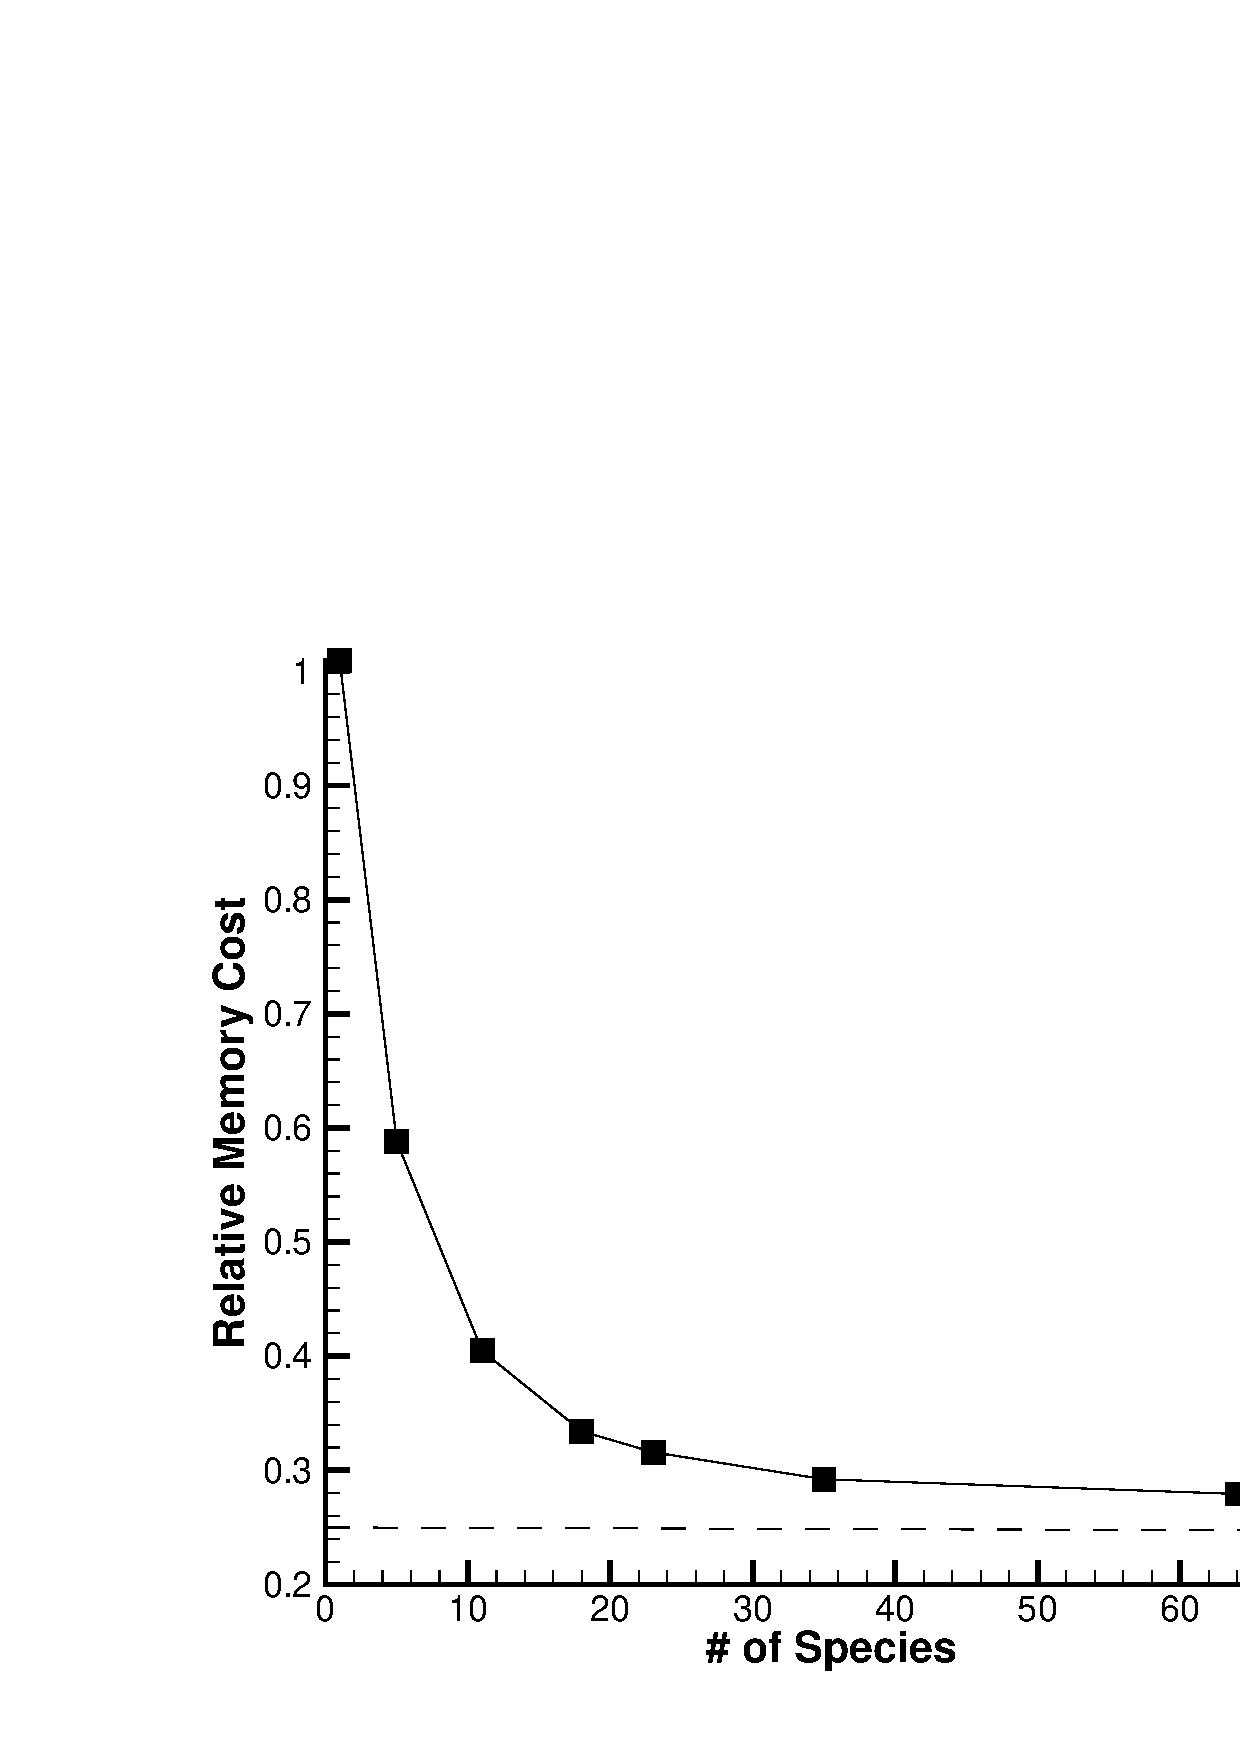
\includegraphics[width=0.45\textwidth]{figures/scitech/mem_req}
    \caption{Memory required convergence study} 
    \vspace{-2em}
    \label{mem_req}
    \end{center} 
\end{figure}
%------------------------------------------------------------------------------%
thus, the relative memory saved by using the decoupled scheme correctly
approaches a factor of 1/4.

\subsection{Cylinder - Computational Cost}
\label{sec:cylinder-comp-cost}

As stated before, the cost of solving the decoupled implicit system should scale
approximately linearly with the number of species, whereas the fully coupled
problem should scale quadratically; thus, the speedup of the implicit solve
should be approximately linear when comparing the decoupled and fully coupled
approaches.  Figure \ref{rel_speedup} shows this to be true for the cylinder test
case, but that the total speedup of the problem is less than that of just
the linear solve.
%------------------------------------------------------------------------------%
\begin{figure}[h]
  \centering
  \includegraphics[width=0.45\textwidth]{figures/scitech/speedup} 
  \caption{ Relative speedup for the decoupled scheme vs. fully coupled scheme.}
  \label{rel_speedup} 
\end{figure}
%------------------------------------------------------------------------------%
The fact that the overall gains are not as large as those for the implicit
solve is due to Amdahl's law: the overall speedup is always limited by the
slowest component.  There are many other factors that scale with the number of
species, especially calculating the species source term and its linearization.
%------------------------------------------------------------------------------%
\begin{figure}[h]
  \centering
  \includegraphics[width=0.5\textwidth]{figures/flow-efficiency/percent-cost.png}
  \caption{Relative Cost of Flow Solver Components for 11-Species}
  \label{fig:percent-cost-cyl}
\end{figure}
%------------------------------------------------------------------------------%
\fref{fig:percent-cost-cyl} shows that jacobian evaluations and computing the
thermo-chemical state have superceded the linear solver as the dominant cost of
the simulation.  The overall speedup of the decoupled scheme over the fully
coupled scheme is constrained by these, and also highlights the sensivity to the
jacobian evaluation frequency.  When the non-linear update is rapidly converging
the residuals, the jacobian is usually updated only one every 10 iterations.
Likewise, when the non-linear update is not resulting a sustained residual
decrease the jacobian is updated every iteration.  This has a large effect on
relative computational efficiency, and poorly converging solutions can be
expected to show less relative speedup between the fully coupled and decoupled
schemes.

\section{15 km/s Flow over Spherically-Capped Cone}
\label{sec:15-kps-sphere-cone}

To ensure that the decoupled scheme is robust and accurate at higher velocities, both the
fully coupled and decoupled approaches were run on a sphere-cone geometry
identical to that presented by Candler et. al. \cite{candler} (10 cm nose
radius, 1.1 m length, 8$^o$ cone angle).  For this case, a simple 64$\times$64
hexahedra grid was constructed, and freestream conditions were set as
$V_{\infty} = 15000\ m/s$, $\rho_{\infty}=0.001\ kg/m^3$, $T_\infty = 200\ K$.
Due to the large reaction rates during the transients at startup, when the
stagnation temperatures are very high, it was necessary to employ the scaling
factor, $\omega_r$ in order to ramp the magnitude of chemical source term.
Ramping was only required in the first 500 iterations, and no scaling was
performed on the source term when the solution was well with the radius of
convergence.

\subsection{Sphere-Cone - Verification of Implementation} 

As with the cylinder test case, the surface pressure and temperature were used
as metrics to determine that both the decoupled and fully coupled approaches
give the same answer when converged to steady-state. The species composition
consisted of N, $\text{N}_2$, O, $\text{O}_2$, NO, N$^+$, $\text{N}_2^+$, O$^+$,
$\text{O}_2^+$, NO$^+$, and electrons, with 22 possible reactions. Figure
\ref{cone_predictions} shows that both methods again yield similar results, and
the high stagnation temperature indicates that this is an inviscid,
one-temperature simulation.  This demonstrates that the decoupled approach is
able to converge to the same solution as the fully coupled solution, in spite of
the chemical reactions proceeding very rapidly due to a high stagnation
temperature.

%------------------------------------------------------------------------------%
\begin{figure}
	\centering
	\begin{subfigure}[b]{0.4\textwidth}
		\centering
		\includegraphics[width=\textwidth]{figures/scitech/surface_pressure_cone}
		\caption{Surface pressure}
		\label{cone_pressure}
	\end{subfigure}
	\begin{subfigure}[b]{0.4\textwidth}
		\centering
		\includegraphics[width=\textwidth]{figures/scitech/surface_temperature_cone}
		\caption{Surface temperature}
		\label{cone_temp}
	\end{subfigure}
  \caption{ Sphere-cone predicted quantities. }
  \label{cone_predictions}
\end{figure}
%------------------------------------------------------------------------------%

\subsection{Sphere-Cone - Convergence Quality}

The limits on the stability of the decoupled scheme derives from introducing
explicitness in creating and destroying species.  By scaling the magnitude of
the chemical source term during the transient phase of the solve, this
instability can be mitigated, and the convergence of decoupled scheme approaches
that of the fully coupled scheme. Scaling of chemical source term was done
identically between the decoupled and fully coupled scheme by ramping the
factor $\omega$ from 0.001 to 1.0 over the first 500 timesteps. Figure
\ref{cone_convergence} shows that the convergence of both schemes progresses
nearly identically, with the decoupled scheme converging in significantly less
computational time and, interestingly, fewer timesteps.
%------------------------------------------------------------------------------%
\begin{figure}
	\centering
	\begin{subfigure}[b]{0.45\textwidth}
		\centering
    \includegraphics[width=\textwidth]{figures/scitech/cone_iteration}
		\caption{Iterations to convergence}
		\label{cone_iterations}
	\end{subfigure}
	\begin{subfigure}[b]{0.45\textwidth}
		\centering
		\includegraphics[width=\textwidth]{figures/scitech/cone_walltime}
    \caption{Computational time to convergence}
		\label{cone_walltime}
	\end{subfigure}
  \caption{ Sphere-cone convergence details. }
  \label{cone_convergence}
\end{figure}
%------------------------------------------------------------------------------%
This demonstrates that the decoupled scheme has significant potential to
improve the efficiency of high-velocity simulations, and that the stiffness of
the source term can be overcome in the presence of large chemical reaction
rates.

\subsection{Sphere Cone - Convergence Improvement with Exact First-Order Linearizations}
\label{sec:sphere-cone-exact-approx-convergence}

An important benefit of implementing an adjoint solver in FUN3D derives from the
requirement of exact linearizations, because the linearizations needed to form
the residual in the adjoint solver can be reused by the flow solver.
Due to the high storage requirements associated with exactly linearizing the
gradient terms in the reconstruction, an approximate Jacobian is used in the
flow solver.  This approximate Jacobian consists of linearizations of the
first-order scheme, as is used to solve the governing equations via defect
correction.  Previously, the reacting gas path employed a Jacobian also, that
approximated the linearizations of the Roe FDS scheme\cite{gnoffo-tp} as
%------------------------------------------------------------------------------%
\begin{equation}
  \rdiff{}{\mU} = 
  \frac{1}{2} \left( \rdiff{c}{\mU} + \rdiff{\tilde{c}}{\mU} \right)
  \label{approx-roe-jac}
\end{equation}
%------------------------------------------------------------------------------%
where $\rdiff{c}{\mU}$ is the linearization of the convective portion of the Roe
FDS scheme, and $\rdiff{\tilde{c}}{\mU}$ is the approximation to the dissipation
term in the Roe RDS scheme, formed by evaluating $\rdiff{c}{\mU}$ with Roe
averaged quantities.  This approximation has been is used by others
\cite{rinaldi2014exact} to mitigate the development time of implementing an
exact linearization of the dissipation term in the Roe FDS scheme, as well the
large computational cost in computing those linearizations at each Jacobian
update.

To demonstrate any benefit of the exact linearization of the Roe FDS scheme on
iterative convergence of the flow solver, the sphere cone case was converged
using both the Jacobian employing exact linearizations of the Roe FDS scheme
flux, and the Jacobian employing the approximation in \eref{approx-roe-jac}.
%------------------------------------------------------------------------------%
\begin{figure}[h]
  \centering
  \includegraphics[width=0.5\textwidth]{figures/flow-efficiency/exact-approx-speedup.png}
  \caption{Relative Speedup Using Exact Linearizations}
  \label{fig:exact-approx-speedup}
\end{figure}
%------------------------------------------------------------------------------%
\fref{fig:exact-approx-speedup} shows that up to a five-species air mixture, the
convergence to steady state is completed in $58\%$ to $90\%$ less simulation
time.  For the 11 species air mixture, involving ionization, the speed up
promptly plateaus, as the additional costs incurred by computing the exact
linearizations supercede the improved iterative convergence.  It can be inferred
from \fref{fig:exact-approx-speedup} that the improvements compounded by the
decoupled scheme, which affords iterative converge similar to the exact fully
coupled scheme, will be significantly faster than the baseline scheme that was
originally implemented in the reacting gas path of FUN3D.

\section{Re-entry Vehicle with Retro-Firing Annular Jet}

The demonstration problem presented in \crefs{chapter-five}{chapter-six}
presents the most challenging problem for the decoupled scheme, due to the
Hydrogen-air combustion.  To verify that the solution is not effected by
employing the decoupled scheme over the fully coupled scheme, the comparison is
made between solutions of the decoupled and fully coupled flow solvers on the
cost function component quantities in \sref{cost-func-components}.  The
freestream conditions in \tref{tab:flow-conditions} were used for this
comparison, along with the plenum conditions in \tref{tab:plenum-conditions}.

\subsection{Annular Jet: Verification of Implementation}
\label{sec:annular-jet-flow-verify}

To determine consistency between the fully coupled and decoupled schemes, the
surface temperature RMS, $T_{RMS}$, and mass flow rate, $\massflow$, were
computed and compared.  Because of the flux limiter sensitivity and poor
relative convergence with finite-rate chemistry discussed in
\sref{sec:frozen-limiter}, the comparision was made for both frozen flow and
flow in chemical non-equilibrium.
%------------------------------------------------------------------------------%
\begin{table}
  \centering
  \begin{tabular}{c|c|c|c}
    Quantity & Decoupled & Fully Coupled & Relative Difference \\
    \hline
    $\massflow$ & 0.8450858226893225E-03 & 0.8450858226893034E-03 & 2.26E-14 \\
    $T_{RMS}$   & 0.1508600871984388E+04 & 0.1508600871984388E+04 & 0
  \end{tabular}
  \caption{Difference with Frozen Chemistry}
  \label{tab:srp-frozen-flow-diff}
\end{table}
%------------------------------------------------------------------------------%
\tref{tab:srp-frozen-flow-diff} shows that, for frozen chemistry, the decoupled
and fully coupled schemes match discretely for surface temperature, and to
within approximately machine precision for the mass flow rate through the
plenum.  The residual was less than $10^{-16}$ for all equations in this
comparison, and only the last digit of both quantities in
\tref{tab:srp-frozen-flow-diff} were changing by the end of the solution.
%------------------------------------------------------------------------------%
\begin{table}
  \centering
  \begin{tabular}{c|c|c|c}
    Quantity & Decoupled & Fully Coupled & Relative Difference \\
    \hline
    $\massflow$ & 0.8448720721551258E-03 & 0.8448720721551088E-03 & 2.01E-14 \\
    $T_{RMS}$   & 0.1545729169703027E+04 & 0.1545720949811712E+04 & 5.32E-06
  \end{tabular}
  \caption{Difference with Finite-Rate Chemistry}
  \label{tab:srp-chem-flow-diff}
\end{table}
%------------------------------------------------------------------------------%
\tref{tab:srp-chem-flow-diff} shows, for reacting chemistry, similar agreement
with regard to the plenum mass flow rate, but poorer agreement of the surface
temperature. Given the varying degrees of convergence shown in
\fref{fig:chem-res-comp}, this difference in surface temperature is not
surprising. At the point the convergence stall, with the residual of all
equations hanging at $\sim 10^{-8}$, only the last nine digits were still
changing.  This indicates that improving the conditioning of the problem, in
order to enable further converge of the flow equation residuals to machine zero,
would likely decrease the relative difference between the fully coupled and
decoupled flow solver schemes.  For engineering applications this difference is
trivial and it has only minimal impact, if any, on the design optimization
procedure.  The effect of the flux limiter sensitivity is much greater on the
design optimzation procedure, and it was found that the using the decoupled
scheme or the fully-coupled scheme in the optimization from \cref{chapter-five}
converged to the same result if the limiter fields were made identical between
the schemes.

\subsection{Annular Jet: Convergence Quality}

Due to startup transients, where reaction rates grew very large as nearly all
$H_2$ and $O_2$, and most of $N_2$, dissociated near the stagnation region, the
source ferm scaling factor, $\omega_r$, was employed for this problem to
maintain stability.  It was empirically determined that the source term scaling
could be removed within the first third of the way to convergence for this
problem.  

%------------------------------------------------------------------------------%
\begin{figure}[h]
  \centering
	\begin{subfigure}[b]{0.45\textwidth}
    \includegraphics[width=\textwidth]{figures/flow-efficiency/dc-gfc-res-chem.png}
    \caption{Finite-Rate Chemistry}
    \label{fig:srp-dc-gfc-res-frozen}
  \end{subfigure}
	\begin{subfigure}[b]{0.45\textwidth}
    \includegraphics[width=\textwidth]{figures/flow-efficiency/dc-gfc-res-frozen.png}
    \caption{Frozen Chemistry}
    \label{fig:srp-dc-gfc-res-chem}
  \end{subfigure}
  \caption{Second-Order Residual Convergence History}
  \label{fig:srp-dc-gfc-res}
\end{figure}
%------------------------------------------------------------------------------%
\fref{fig:srp-dc-gfc-res} shows a comparsion of the residual convergence for the
fully coupled schemes, with exact first-order linearizations and the
approximations described in \sref{sec:sphere-cone-exact-approx-convergence}, and
the decoupled scheme.  The comparing
\frefs{fig:srp-dc-gfc-res-frozen}{fig:srp-dc-gfc-res-chem}, there is a stark
difference both the minimum residual convergence and the ``smoothness'' of the
convergence profile.  When the no chemical source terms are present (frozen
flow), the flow equation residuals are able to be converged to $ < 10^{-16}$,
with very few high-frequency errors encountered after the limiter is frozen at
4000 iterations.  When chemistry is engaged, the convergence of the flow
equation residuals stalls at approximately $10^{-8}$, and there are a large
number of high-frequency errors in the solution updates after the limiter is
frozen, due to the frozen limiter needing to be re-evaluated.
\fref{fig:srp-dc-gfc-res-chem} shows that the decoupled scheme is more
sensitive to the frozen limiter than either of the fully coupled schemes.  This
is not overly surprising, since the re-evaluation of the flux limiter is
sensitive to subtle changes in the species densities, and the decoupled
scheme Jacobians have a large number of approximations with regard to species
density linearizations.  As show in \sref{sec:annular-jet-flow-verify}, the
impact of this poor convergence quality on the quantities of interest is
minimal, and this degree of convergence is more than sufficient to obtain the
sensitivity gradients required in design optimization.

\subsection{Annular Jet: Relative Speedup}

The computational cost of decoupled scheme and fully coupled scheme with exact
first-order linearizations is compared to the previously implemented fully coupled
scheme with approximate first-order linearizations.
For flow with frozen chemistry, show in \fref{fig:srp-dc-gfc-res-frozen},
the solution is considered converged when the flow residual $L_2$ norm is less
than $10^{-16}$, and the relative speedup is shown in
\tref{tab:srp-rel-speedup-frozen}
%------------------------------------------------------------------------------%
\begin{table}[h]
  \centering
  \begin{tabular}{c|c|c}
    Scheme & Time (s) & Speedup \\
    \hline
    Fully Coupled (Approximate) & 348.6 & 1.0 (baseline) \\
    Fully Coupled (Exact)       & 265.6 & 1.31 \\
    Decoupled                   & 138.7 & 2.51
  \end{tabular}
  \caption{Relative Speedup for Frozen Chemistry}
  \label{tab:srp-rel-speedup-frozen}
\end{table}
%------------------------------------------------------------------------------%
The decoupled scheme is considerably faster than either of the two fully coupled
schemes, and the improved iterative convergence afforded by the exact
linearizations prove valuable to the fully coupled scheme for this case, where
the residuals can be converged an additional 10 orders of magnitude after the
limiter is frozen.  Determining the relative speedup is difficult for the
schemes in \fref{fig:srp-dc-gfc-res-chem}, where finite-rate chemistry is
engaged, due to noise in the convergence history.  Because of this, total
solution time is used in lieu of a residual convergence level to compute the
relative speedup in \tref{tab:srp-rel-speedup-chem}
%------------------------------------------------------------------------------%
\begin{table}[h]
  \centering
  \begin{tabular}{c|c|c}
    Scheme & Time (s) & Speedup \\
    \hline
    Fully Coupled (Exact)       & 280.6 & 1.0 (baseline) \\
    Fully Coupled (Approximate) & 270.4 & 1.04 \\
    Decoupled                   & 168.6 & 1.66
  \end{tabular}
  \caption{Relative Speedup for Finite-Rate Chemistry}
  \label{tab:srp-rel-speedup-chem}
\end{table}
%------------------------------------------------------------------------------%
The gains associated with chemistry engaged are significantly less than those
with frozen chemistry for this annular jet case.  Due to stalled convergence,
there is no clear advantage of using exact linearizations over approximate
linearizations in the fully coupled scheme, although the relative savings of use
approximate linearizations are almost negligible ($4\%$).  The decoupled scheme
is 66\% faster than the exact, fully coupled scheme, and the difference between
this result and the frozen flow result is the poorer iterative convergence
quality.  As discussed in \sref{sec:cylinder-comp-cost}, the the frequency of
the jacobian evaulation is tied to the decrease in the residual from each
non-linear solution update.  Due to the poorer convergence seen in
\fref{fig:srp-dc-gfc-res-chem}, the jacobian is reevaluated at each iteration.
This significantly diminishes the relative speedup of the decoupled scheme.
This causes the jacobian update to become a bottleneck in computational time
required, and the additional cost of computing chemical source term and its
jacobian at each timestep reduces the relative speedup further in comparison to
frozen flow.


\chapter{Relative Efficiency of Decoupled Adjoint Solver}
\label{chapter-nine}

At this point, the reacting gas adjoint in FUN3D has been utilized to obtain
sensitivity information needed to drive design optimization, and the
sensitivities of the fully coupled scheme have been validated against complex
Frechet derivatives for accuracy.  A key point of this study is to demonstrate
the increase computational efficiency and relative memory saving of using a
decoupled variable set for the flow and adjoint solvers, instead of a fully
coupled variable set.  This chapter details the benefits of applying the
decoupled adjoint solver over the fully coupled solver for the annular jet
demonstration problem.

\section{Verification of Consistency}
\label{adj-consistency}

Section \ref{block-jacobi-decoupling} showed in detail that, in the adjoint,
changing from the fully coupled variable and equation sets to the decoupled
variable and equation sets could be accomplished by a series of matrix
transformations on the Jacobian.  This transformation is equivalent to a left
and right preconditioning of the fully coupled scheme, enabling the reuse of the
approximate Jacobians used by the flow solver.  Provided the adjoint system is
well conditioned and convergence is sufficient, preconditioning should not
affect the final adjoint solution; thus, we expect to recover the exact same
solution from both the fully coupled and decoupled adjoint schemes.

The 5 $km/s$ spanwise cylinder case from \sref{sec:5-kps-cylinder} and the 15
$km/s$ sphere cone case from \sref{sec:15-kps-sphere-cone} are re-examined here
to determine the consistency of the adjoint solution computed by the fully
coupled schemes.  In this case, the sensitivity of the drag coefficient, $C_D$
to the angle of attack, $\alpha$, is computed by both schemes and compared.
%------------------------------------------------------------------------------%
\begin{table}[h]
  \centering
  \begin{tabular}{c|c|c|c}
    Case & Decoupled Sensitivity & Fully Coupled Sensitivity & Rel. Diff\\
    \hline
    Cylinder    &  0.764409218044021E-07 &  0.764409218054372E-07 & 1E-11 \\
    Sphere-Cone & -0.877773486565165E-02 & -0.877773486565157E-02 & 2E-14
  \end{tabular}
  \caption{Angle of attack sensitivity relative difference.}
  \label{tab:cylinder-adj-diff}
\end{table}
%------------------------------------------------------------------------------%
\tref{tab:cylinder-adj-diff} shows that the solutions match discretely to at
least 11 digits, and is indicative that the decoupled iterative mechanism can be
used to compute the adjoint solution without changing the result.  It should be
recognized here that, in the continuous sense, the drag on a cylinder is
independent of angle of attack; however, in the discrete sense of this grid,
which is only a half-body cylinder, there is a minimal dependence between angle
of attack and drag.

For the annular jet demonstration problem, the sensitivities computed in
\tref{tab:react-deriv-check} were checked to verify that decoupled and fully
coupled adjoint solutions matched to give the same sensitivity.
%------------------------------------------------------------------------------%
\begin{table}[h]
  \centering
  \begin{tabular}{c|c|c|c}
    Design Variable & Decoupled Sensitivity & Fully Coupled Sensitivity & Rel. Diff\\
    \hline
    $P_{p,o}$ & -0.11081315601976E-06 & -0.11081315649260E-06 & 4E-9  \\
    $T_{p,o}$ &  0.19089941243495E-03 &  0.19089941237390E-03 & 3E-10 \\
    $\fa$     & -0.28035409093945E-01 & -0.28035409045530E-01 & 1E-9
  \end{tabular}
  \caption{Annular jet plenum sensitivity relative difference.}
  \label{tab:srp-adj-diff}
\end{table}
%------------------------------------------------------------------------------%
\tref{tab:srp-adj-diff} also gives excellent agreement between the decoupled and
fully coupled adjoint schemes.  Examining the differences of sensitivities in
\trefs{tab:cylinder-adj-diff}{tab:srp-adj-diff}, it is clear
that the absolute difference is almost always on the order of $10^{-15}$ each
case.  Since double precision was used in all floating point operations for
these cases, this is consistent with the level of precision used.

As a note on robustness, none of the stability issues found in the decoupled
flow solver have been observed for the decoupled adjoint scheme.  The
non-linear nature of the chemical source term was the primary stability concern
in the decoupled flow solver, since the explicitness introduced by the decoupled
mass fraction update exacerbates CFL restrictions.  These problems disappear in
the adjoint equations, since it is a linear system being solved instead of a
highly non-linear one.  The full stability and convergence properties of the
fully coupled adjoint solver were recovered by the decoupled adjoint solver, and
it is therefore concluded that there is no advantage of solving the adjoint
system in a fully coupled manner.

\section{Relative Memory Savings and Speedup}
\label{sec:adj-cost-mem-savings}

The computational cost of the solution process in the adjoint can be greatly
improved by storing the exact linearizations of the discrete flow solver
equations, as discussed in \sref{sec:2nd-order-mem-cost}.  For a second order
scheme 
%------------------------------------------------------------------------------%
\begin{figure}[h]
	\begin{subfigure}[b]{0.45\textwidth}
    \centering
    \includegraphics[width=\textwidth]{figures/adj-efficiency/adj-recompute.png}
    \caption{Linearizations always recomputed}
    \label{fig:always-recompute}
  \end{subfigure}
	\begin{subfigure}[b]{0.45\textwidth}
    \centering
    \includegraphics[width=\textwidth]{figures/adj-efficiency/adj-stored.png}
    \caption{Linearizations stored}
    \label{fig:stored}
  \end{subfigure}
  \caption{Simulation time comparison.}
  \label{fig:sim-time-comp}
\end{figure}
%------------------------------------------------------------------------------%
\fref{fig:sim-time-comp} shows the comparison of the fully coupled adjoint and 
decoupled adjoint time to solution with the two mechanisms for computing the
exact linearizations.  \tref{tab:srp-rel-speedup} shows that the speedup of
decoupled scheme is only truly realized when the exact linearizations are store,
rather than recomputed at each timestep. 
%------------------------------------------------------------------------------%
\begin{table}[h]
  \centering
  \begin{tabular}{c|c|c|c}
    Scheme & Linearizations & Time to Convergence (s) & Speedup \\
    \hline
    Fully Coupled & Recomputed  & 309.4 & 1.0 (baseline)\\
    Decoupled     & Recomputed  & 244.2 & 1.27 \\
    Fully Coupled & Stored      & 61.22 & 5.05 \\
    Decoupled     & Stored      & 18.69 & $\mathbf{16.6}$ \\
  \end{tabular}
  \caption{Relative speedup.}
  \label{tab:srp-rel-speedup}
\end{table}
%------------------------------------------------------------------------------%
This is because computing the exact linearizations in the adjoint is the
dominant cost.  The comparison between storing the linearizations and
recomputing them is somewhat unfair, as the ability to store the full Jacobian
of the second order reconstruction may not be possible, due to memory
constraints.  That said, a significant advantage of the decoupled scheme over
the fully coupled scheme is the memory savings offered by the LHS Jacobian
sparsity. It was show in \sref{sec:predicted-cost-mem-savings} that the
predicted memory savings for a infinite number of species is $1/7$ for a
hexahedra grid where the average number of neighbors is 6.  Unfortunately, the
storage requirements for the exact linearizations will not change between the
decoupled and fully coupled schemes; however, as the average number of neighbors
in the grid increases, the relative memory savings will also increase.  To
effectively demonstrate this, the amount of memory required by the adjoint
solver with the exact linearizations stored was determined for each mesh of the
refinement study in \sref{sec:mesh-refinement-study}.
%------------------------------------------------------------------------------%
\begin{figure}[h]
  \centering
	\begin{subfigure}[b]{0.45\textwidth}
    \centering
    \includegraphics[width=\textwidth]{figures/adj-efficiency/mem-req-srp.png}
    \caption{Absolute memory required}
    \label{fig:abs-mem-req}
  \end{subfigure}
	\begin{subfigure}[b]{0.45\textwidth}
    \centering
    \includegraphics[width=\textwidth]{figures/adj-efficiency/mem-rel-savings.png}
    \caption{Relative memory required}
    \label{fig:relative-mem-req}
  \end{subfigure}
  \caption{Memory required to store full linearizations.}
  \label{fig:srp-mem-req}
\end{figure}
%------------------------------------------------------------------------------%
\fref{fig:srp-mem-req} is somewhat encouraging a face value, since it was
possible to store the exact linearizations for the 3.1 million node mesh,
simulating a 9-species hydrogen air mixture.  \fref{fig:abs-mem-req} show, as
expected, that the memory requirements for both the fully coupled and decoupled
schemes scale directly with the number of mesh points.  The relative savings for
this case are nowhere near the predicted $1/7$ value, because the exact
linearizations require significantly more memory than anything else store in the
adjoint solver.  That said, the $\sim 20\%$ decrease in memory required by the
decoupled adjoint solver is significant, since the ability to store the exact
linearizations is a binary problem: either there is enough memory or there is
not.  The increased savings are as important as the speedup, if not more, since
the decoupled scheme can facilitate larger problems to be solved with greater
than an order of magnitude increase in computational efficiency, if the exact
linearizations can be stored.

\chapter{Concluding Remarks}
\label{chapter-ten}

An implicit, decoupled scheme has been implemented in the reacting gas path of
the FUN3D flow solver, and an adjoint solver employing a fully coupled and
decoupled scheme has also been implemented.  The sensitivity dervatives provided
by the adjoint solver have been verified using a complex-variable approach, and
a sample inverse optimization and direct optimization was completed on a
hypersonic re-entry vehicle geometry that employed a retro-firing annular jet.

The consistency and robustness of decoupling the variable sets in the flow
solver was examined.  It was found that the decoupled scheme only exhibited
stability issues when the chemical source term was very large, due to large
reaction rates.  This stability issue was mitigated by multiplying the chemical
source term uniformly by scaling term, which could be ramped from zero to one
over the course of the simulation.  Provided that the ramping was completed, the
true steady-state solution, done without ramping, was recovered.  The
consistency of the solutions computed by the fully coupled and decoupled methods
was found to match discretely for surface temperature and pressure, and to
within $10^{-4}$ for mass fractions on the stagnation line of a spanwise
cylinder case in a $5 km/s$ flow.  It was also determined that this difference
in mass fraction was reduced with mesh spacing.

The decoupled adjoint scheme demonstrated here is a significant improvement to
the state of the art in the field of sensitivity analysis for reacting flows.
The decreased memory and computational costs afforded by solving a decoupled
dependent variable set in the adjoint solver enable a speedup greater than an
order of magnitude for some cases.  



%%---------------------------------------------------------------------------%%
%%  Bibliography 

\bibliography{KyleThompson-thesis}{}
\bibliographystyle{plain}

%%---------------------------------------------------------------------------%%
% Appendices
\appendix

\chapter{Derivations}

\section{Decoupled Flux Derivation}

For the Roe flux difference splitting scheme, the species mass fluxes are given by
%
\begin{equation}
	F_{\rho_s} = \frac{\rho_s^L\overline{U}^L+\rho_s^R\overline{U}^R}{2}
	-\frac{\tilde{c}_s(\lambda_1 dv_1 + \lambda_2 dv_2)+\lambda_3 dv_{3_s}}{2} \label{species_mass} \\
\end{equation}
\begin{align}	
		dv_1 &= \frac{p^R-p^L+\tilde{\rho} \tilde{a} (\overline{U}^R-\overline{U}^L)}{\tilde{a}^2} \\
		dv_2 &= \frac{p^R-p^L-\tilde{\rho} \tilde{a} (\overline{U}^R-\overline{U}^L)}{\tilde{a}^2} \\
		dv_{3_s} &= \frac{\tilde{a}^2 (\rho_s^R-\rho_s^L)- \tilde{c}_s (p^R-p^L)}{\tilde{a}^2}
\end{align}
\begin{align}
	\lambda_1 = \mid\mathbf{\overline{U}}+\tilde{a} \mid,\quad 
	\lambda_2 = \mid \mathbf{\overline{U}}-\tilde{a} \mid,\quad 
	\lambda_3 =  \mid \mathbf{\overline{U}} \mid
\end{align}
%
where the $\tilde{}$ notation signifies a Roe-averaged quantity, given by:
%
\begin{gather}
	\mathbf{\tilde{U}} =w\mathbf{\tilde{U}}^L+(1-w)\mathbf{\tilde{U}}^R \\
	w = \frac{\tilde{\rho}}{\tilde{\rho}+\rho^R} \\
	\tilde{\rho} = \sqrt{\rho^R\rho^L}
\end{gather}
%
The species mass fluxes must sum to the total mass flux; thus, the total mixture mass flux is given as
%
\begin{equation}
\label{total_mass}
	F_\rho = \sum\limits_{s}{F_{\rho_s}} = \frac{\rho^L\overline{U}^L+\rho^R\overline{U}^R}{2}
	-\frac{\tilde{c}_s(\lambda_1 dv_1 + \lambda_2 dv_2)+\lambda_3 dv_3}{2}
\end{equation}
\begin{equation}
	dv_3 = \frac{\tilde{a}^2 (\rho^R-\rho^L)-(p^R-p^L)}{\tilde{a}^2}
\end{equation}
%
Multiplying Eq.~(\ref{total_mass}) by the Roe-averaged mass fraction and
substituting it into Eq.~(\ref{species_mass}) results in:
%
\begin{equation}
\label{unsimp_sp_flux}
	F_{\rho_s} =\tilde{c}_s F_\rho + \frac{(c_s^L-\tilde{c}_s)\rho^L(\overline{U}^L+\mid \tilde{U}\mid)}{2}
	+ \frac{(c_s^R-\tilde{c}_s)\rho^R(\overline{U}^R-\mid \tilde{U}\mid)}{2}
\end{equation}
%
It should be noted here that the Roe-averaged normal velocity, $\tilde{U}$,
requires an entropy correction in the presence of strong shocks\cite{harten}.
This correction has no dependence on the species mass fractions; therefore,
it does not change the form of the Jacobian for this decoupled scheme. The
notation can be further simplified by defining the normal velocities as follows:
%
\begin{equation} \label{lambda_pm} \lambda^+ = \frac{\overline{U}^L+\mid
  \tilde{U}\mid}{2}, \quad \lambda^- = \frac{\overline{U}^R-\mid
  \tilde{U}\mid}{2} \end{equation}
%
Finally, substituting Eq.~(\ref{lambda_pm}) into Eq.~(\ref{unsimp_sp_flux})
yields the final result for calculating the species flux in the decoupled
system:
%
\begin{equation} \label{sp_flux} F_{\rho_s} =\tilde{c}_s F_\rho +
  (c_s^L-\tilde{c}_s)\rho^L\lambda^+ + (c_s^R-\tilde{c}_s)\rho^R\lambda^-
\end{equation}
%
Forming the convective contributions to the Jacobians is straightforward.
Because the $\mathbf{U}'$ level variables are constant, only the left, right,
and Roe-averaged state mass fractions vary.  Differentiating Eq.~(\ref{sp_flux})
with respect to the mass fraction, $c_s$, the left and right state contributions
are
%
\begin{gather} \frac{\partial F_{\rho_s}}{\partial c^L_s} =
  wF_\rho+(1-w)\rho^L\lambda^+ - w\rho^R\lambda^- \\ \frac{\partial
    F_{\rho_s}}{\partial c^R_s} = (1-w)F_\rho+(w-1)\rho^L\lambda^+ +
    w\rho^R\lambda^- \end{gather}
%
Because there is no dependence between species in decoupled convective
formulation, the Jacobian block elements are purely diagonal for the convective
contributions, of the form
%
\begin{equation} \begin{pmatrix} \frac{\partial F_{\rho_1}}{\partial c_1} & & 0
    \\ & \ddots &  \\ 0 & & \frac{\partial F_{\rho_{ns}}}{\partial c_{ns}}
  \end{pmatrix} \end{equation}


%%---------------------------------------------------------------------------%%
\backmatter

\end{document}
